% Options for packages loaded elsewhere
\PassOptionsToPackage{unicode}{hyperref}
\PassOptionsToPackage{hyphens}{url}
\documentclass[
  ignorenonframetext,
]{beamer}
\newif\ifbibliography
\usepackage{pgfpages}
\setbeamertemplate{caption}[numbered]
\setbeamertemplate{caption label separator}{: }
\setbeamercolor{caption name}{fg=normal text.fg}
\beamertemplatenavigationsymbolsempty
% remove section numbering
\setbeamertemplate{part page}{
  \centering
  \begin{beamercolorbox}[sep=16pt,center]{part title}
    \usebeamerfont{part title}\insertpart\par
  \end{beamercolorbox}
}
\setbeamertemplate{section page}{
  \centering
  \begin{beamercolorbox}[sep=12pt,center]{section title}
    \usebeamerfont{section title}\insertsection\par
  \end{beamercolorbox}
}
\setbeamertemplate{subsection page}{
  \centering
  \begin{beamercolorbox}[sep=8pt,center]{subsection title}
    \usebeamerfont{subsection title}\insertsubsection\par
  \end{beamercolorbox}
}
% Prevent slide breaks in the middle of a paragraph
\widowpenalties 1 10000
\raggedbottom
\AtBeginPart{
  \frame{\partpage}
}
\AtBeginSection{
  \ifbibliography
  \else
    \frame{\sectionpage}
  \fi
}
\AtBeginSubsection{
  \frame{\subsectionpage}
}
\usepackage{iftex}
\ifPDFTeX
  \usepackage[T1]{fontenc}
  \usepackage[utf8]{inputenc}
  \usepackage{textcomp} % provide euro and other symbols
\else % if luatex or xetex
  \usepackage{unicode-math} % this also loads fontspec
  \defaultfontfeatures{Scale=MatchLowercase}
  \defaultfontfeatures[\rmfamily]{Ligatures=TeX,Scale=1}
\fi
\usepackage{lmodern}
\ifPDFTeX\else
  % xetex/luatex font selection
\fi
% Use upquote if available, for straight quotes in verbatim environments
\IfFileExists{upquote.sty}{\usepackage{upquote}}{}
\IfFileExists{microtype.sty}{% use microtype if available
  \usepackage[]{microtype}
  \UseMicrotypeSet[protrusion]{basicmath} % disable protrusion for tt fonts
}{}
\makeatletter
\@ifundefined{KOMAClassName}{% if non-KOMA class
  \IfFileExists{parskip.sty}{%
    \usepackage{parskip}
  }{% else
    \setlength{\parindent}{0pt}
    \setlength{\parskip}{6pt plus 2pt minus 1pt}}
}{% if KOMA class
  \KOMAoptions{parskip=half}}
\makeatother
\usepackage{longtable,booktabs,array}
\newcounter{none} % for unnumbered tables
\usepackage{calc} % for calculating minipage widths
\usepackage{caption}
% Make caption package work with longtable
\makeatletter
\def\fnum@table{\tablename~\thetable}
\makeatother
\usepackage{graphicx}
\makeatletter
\newsavebox\pandoc@box
\newcommand*\pandocbounded[1]{% scales image to fit in text height/width
  \sbox\pandoc@box{#1}%
  \Gscale@div\@tempa{\textheight}{\dimexpr\ht\pandoc@box+\dp\pandoc@box\relax}%
  \Gscale@div\@tempb{\linewidth}{\wd\pandoc@box}%
  \ifdim\@tempb\p@<\@tempa\p@\let\@tempa\@tempb\fi% select the smaller of both
  \ifdim\@tempa\p@<\p@\scalebox{\@tempa}{\usebox\pandoc@box}%
  \else\usebox{\pandoc@box}%
  \fi%
}
% Set default figure placement to htbp
\def\fps@figure{htbp}
\makeatother
\setlength{\emergencystretch}{3em} % prevent overfull lines
\providecommand{\tightlist}{%
  \setlength{\itemsep}{0pt}\setlength{\parskip}{0pt}}
% Slide layout defaults for warning-clean scientific decks.
\usepackage{etoolbox}
\IfFileExists{xurl.sty}{\usepackage{xurl}}{}
\IfFileExists{seqsplit.sty}{\usepackage{seqsplit}}{\newcommand{\seqsplit}[1]{#1}}
\protected\def\breakseq#1{\seqsplit{#1}}
\protected\def\breaktt#1{\begingroup\ttfamily\seqsplit{#1}\endgroup}
\setlength{\emergencystretch}{6em}
\tolerance=5000
\hbadness=10000
\hfuzz=1pt
\setlength{\tabcolsep}{2pt}
\AtBeginEnvironment{longtable}{\tiny\renewcommand{\arraystretch}{0.86}\setlength{\tabcolsep}{1pt}}
\AtBeginEnvironment{tabular}{\tiny\renewcommand{\arraystretch}{0.86}\setlength{\tabcolsep}{1pt}}

% Natbib and cross-reference fallbacks — slides don't load natbib
% or cleveref, but combined-PDF manuscript prose may emit these
% commands. The fallback renders citations as a bracketed key list
% and cross-references as detokenized labels so slides don't fail on
% undefined control sequences or raw underscores. \providecommand is
% a no-op if packages load later.
\providecommand{\citep}[1]{[#1]}
\providecommand{\citet}[1]{#1}
\providecommand{\citealp}[1]{#1}
\providecommand{\citeauthor}[1]{#1}
\providecommand{\citeyear}[1]{#1}
\providecommand{\cref}[1]{\texttt{\detokenize{#1}}}
\providecommand{\Cref}[1]{\texttt{\detokenize{#1}}}
\usepackage{bookmark}
\IfFileExists{xurl.sty}{\usepackage{xurl}}{} % add URL line breaks if available
\urlstyle{same}
% fallback for those not using the hyperref driver hyperxmp:
\makeatletter
\@ifundefined{xmpquote}{\newcommand{\xmpquote}[1]{#1}}{}
\makeatother
\hypersetup{
  hidelinks,
  pdfcreator={LaTeX via pandoc}}

\author{\texorpdfstring{}{}}
\date{}

\begin{document}

\section{Results}\label{sec:results}

\begin{frame}[fragile,allowframebreaks]{Candidate Outcome}
\protect\phantomsection\label{sec:candidate-outcome}
The generated loop selected \texttt{exp-mlp-tanh-64}
(\breaktt{One-hidden-layer\ tanh\ MLP}, \texttt{MLP}) after evaluating
\texttt{4} candidate(s) from a proposed set of \texttt{5}. The
\breaktt{nearest\_centroid\_baseline} (\breaktt{nearest-centroid})
baseline reached \texttt{82.6\%} \texttt{test\_accuracy}, while the
selected candidate reached \texttt{89.4\%}, an absolute change of
\texttt{6.8\%}. The selected model has \texttt{50890} parameters. The
transformer-candidate evaluated flag is \texttt{true}, and the candidate
budget exhausted flag is \texttt{true}, which means the ledger records
\texttt{1} deferred proposal(s) rather than expanding the run
automatically.

The benchmark score is \texttt{1}. That score is not a model-quality
claim by itself; it is a compact grading artifact for the methods
contract: metric improvement, budget compliance, offline execution, and
selected-candidate recording. Rank-stability diagnostics report that the
selected candidate is top ranked in \texttt{72.5\%} of deterministic
bootstrap resamples, with runner-up \texttt{exp-mlp-relu-32}. The
candidate score figure is registered as @fig:ml\_candidate\_scores, the
confusion matrix as @fig:ml\_confusion\_matrix, the per-class diagnostic
as @fig:ml\_per\_class\_accuracy, the learning curves as
@fig:ml\_learning\_curves, the complexity diagnostic as
@fig:ml\_complexity\_accuracy, the selected-candidate error examples as
@fig:mnist\_error\_examples, the candidate lifecycle diagnostic as
@fig:autoresearch\_candidate\_lifecycle, rank stability as
@fig:ml\_candidate\_rank\_stability, the training-dynamics diagnostic as
@fig:ml\_training\_dynamics, the final readiness matrix as
@fig:autoresearch\_stage\_matrix, and the process closure as
@fig:autoresearch\_closure\_flow.

\begin{longtable}[]{@{}lllll@{}}
\caption{Candidate accuracy intervals from
\protect\breaktt{output/data/ml\_candidate\_intervals.json}; intervals
describe the fixed local test
split.}\label{tbl:candidate-intervals}\tabularnewline
\toprule\noalign{}
Candidate & Status & Correct/test & Accuracy & Wilson 95\% interval \\
\midrule\noalign{}
\endfirsthead
\toprule\noalign{}
Candidate & Status & Correct/test & Accuracy & Wilson 95\% interval \\
\midrule\noalign{}
\endhead
baseline & baseline & 413/500 & 82.6\% & 79.0\% to 85.7\% \\
softmax linear & rejected & 441/500 & 88.2\% & 85.1\% to 90.7\% \\
mlp relu 32 & rejected & 443/500 & 88.6\% & 85.5\% to 91.1\% \\
tiny patch attention & rejected & 152/500 & 30.4\% & 26.5\% to 34.6\% \\
mlp tanh 64 & accepted & 447/500 & 89.4\% & 86.4\% to 91.8\% \\
\bottomrule\noalign{}
\end{longtable}

\begin{longtable}[]{@{}
  >{\raggedright\arraybackslash}p{(\linewidth - 8\tabcolsep) * \real{0.2000}}
  >{\raggedright\arraybackslash}p{(\linewidth - 8\tabcolsep) * \real{0.2000}}
  >{\raggedright\arraybackslash}p{(\linewidth - 8\tabcolsep) * \real{0.2000}}
  >{\raggedright\arraybackslash}p{(\linewidth - 8\tabcolsep) * \real{0.2000}}
  >{\raggedright\arraybackslash}p{(\linewidth - 8\tabcolsep) * \real{0.2000}}@{}}
\caption{Candidate rank-stability table from
\protect\breaktt{output/data/ml\_candidate\_rank\_stability.json};
frequencies are deterministic local bootstrap
summaries.}\label{tbl:candidate-rank-stability}\tabularnewline
\toprule\noalign{}
\begin{minipage}[b]{\linewidth}\raggedright
Candidate
\end{minipage} & \begin{minipage}[b]{\linewidth}\raggedright
Observed rank
\end{minipage} & \begin{minipage}[b]{\linewidth}\raggedright
Top-rank frequency
\end{minipage} & \begin{minipage}[b]{\linewidth}\raggedright
Mean rank
\end{minipage} & \begin{minipage}[b]{\linewidth}\raggedright
Accuracy
\end{minipage} \\
\midrule\noalign{}
\endfirsthead
\toprule\noalign{}
\begin{minipage}[b]{\linewidth}\raggedright
Candidate
\end{minipage} & \begin{minipage}[b]{\linewidth}\raggedright
Observed rank
\end{minipage} & \begin{minipage}[b]{\linewidth}\raggedright
Top-rank frequency
\end{minipage} & \begin{minipage}[b]{\linewidth}\raggedright
Mean rank
\end{minipage} & \begin{minipage}[b]{\linewidth}\raggedright
Accuracy
\end{minipage} \\
\midrule\noalign{}
\endhead
softmax linear & 3 & 4.2\% & 2.554 & 88.2\% \\
mlp relu 32 & 2 & 23.3\% & 2.130 & 88.6\% \\
tiny patch attention & 4 & 0.0\% & 4.000 & 30.4\% \\
mlp tanh 64 & 1 & 72.5\% & 1.316 & 89.4\% \\
\bottomrule\noalign{}
\end{longtable}
\end{frame}

\begin{frame}[allowframebreaks]{Run-Derived Figures}
\protect\phantomsection\label{sec:run-derived-figures}
\begin{figure}
\centering
\pandocbounded{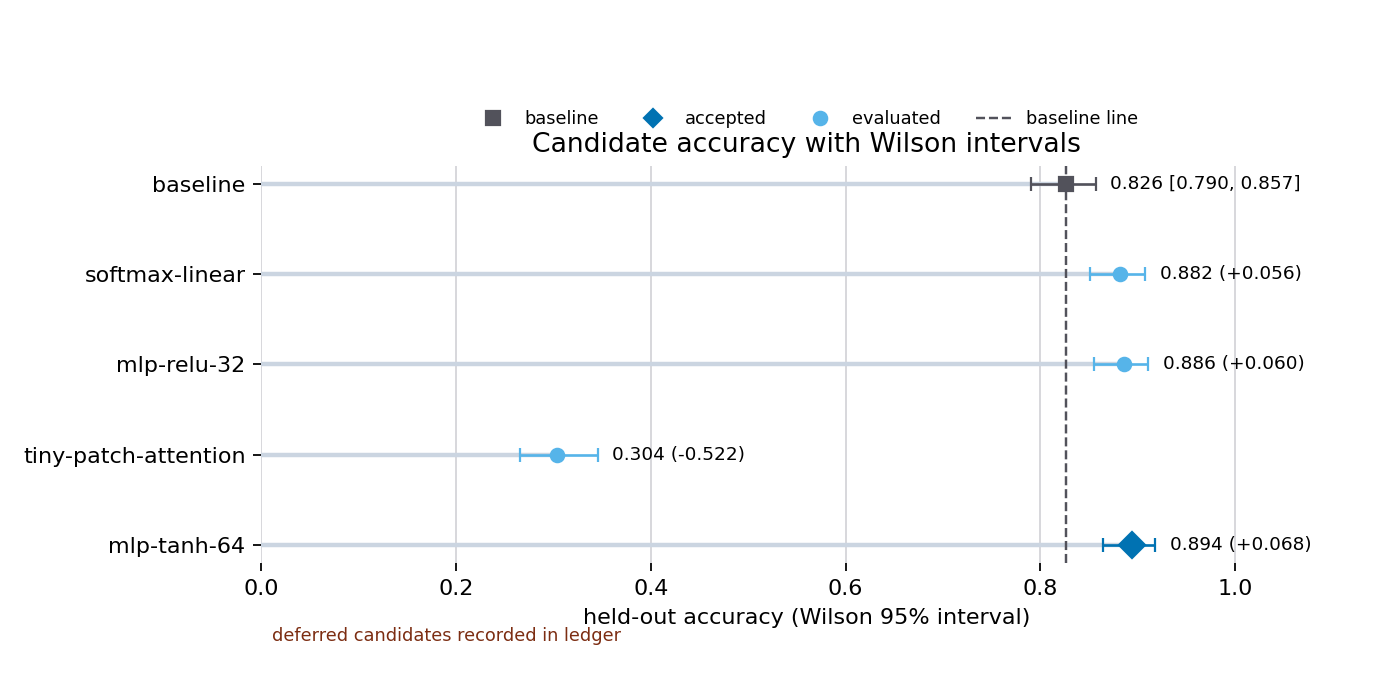
\includegraphics[keepaspectratio,alt={Held-out accuracy with Wilson intervals for the baseline and evaluated candidates from output/data/ml\_candidate\_intervals.json; accepted candidate exp-mlp-tanh-64 improves accuracy from 82.6\% to 89.4\% on the fixed subset, with deferred proposals kept in the candidate ledger. Generation method: Lollipop accuracy comparison with Wilson interval error bars and direct labels. Registry metadata records the generation method, source artifact, and claim boundary for validation.}]{../figures/ml_candidate_scores.png}}
\caption{Held-out accuracy with Wilson intervals for the baseline and
evaluated candidates from output/data/ml\_candidate\_intervals.json;
accepted candidate exp-mlp-tanh-64 improves accuracy from 82.6\% to
89.4\% on the fixed subset, with deferred proposals kept in the
candidate ledger. Generation method: Lollipop accuracy comparison with
Wilson interval error bars and direct labels. Registry metadata records
the generation method, source artifact, and claim boundary for
validation.}\label{fig:ml_candidate_scores}
\end{figure}

\begin{figure}
\centering
\pandocbounded{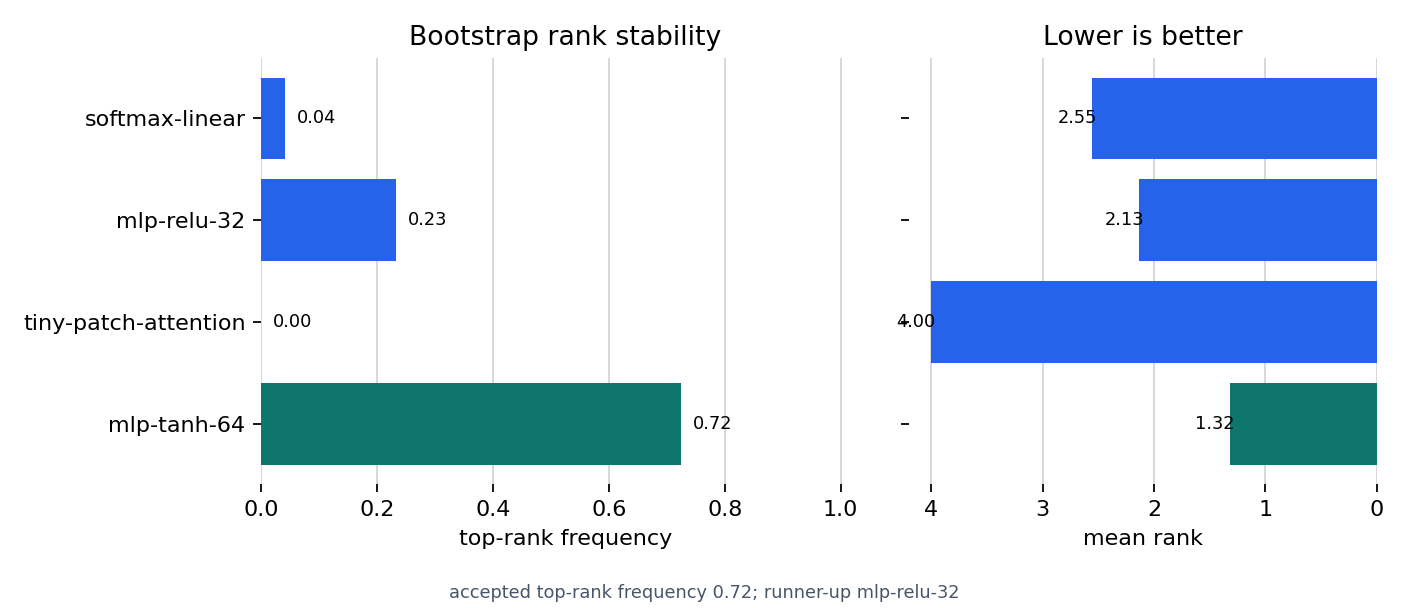
\includegraphics[keepaspectratio,alt={Rank-stability summary for exp-mlp-tanh-64 from output/data/ml\_candidate\_rank\_stability.json; deterministic local bootstrap resampling shows how often each evaluated candidate ranks first under the fixed test split. Generation method: Bootstrap top-rank frequency and mean-rank comparison. Registry metadata records the generation method, source artifact, and claim boundary for validation.}]{../figures/ml_candidate_rank_stability.png}}
\caption{Rank-stability summary for exp-mlp-tanh-64 from
output/data/ml\_candidate\_rank\_stability.json; deterministic local
bootstrap resampling shows how often each evaluated candidate ranks
first under the fixed test split. Generation method: Bootstrap top-rank
frequency and mean-rank comparison. Registry metadata records the
generation method, source artifact, and claim boundary for
validation.}\label{fig:ml_candidate_rank_stability}
\end{figure}

\begin{figure}
\centering
\pandocbounded{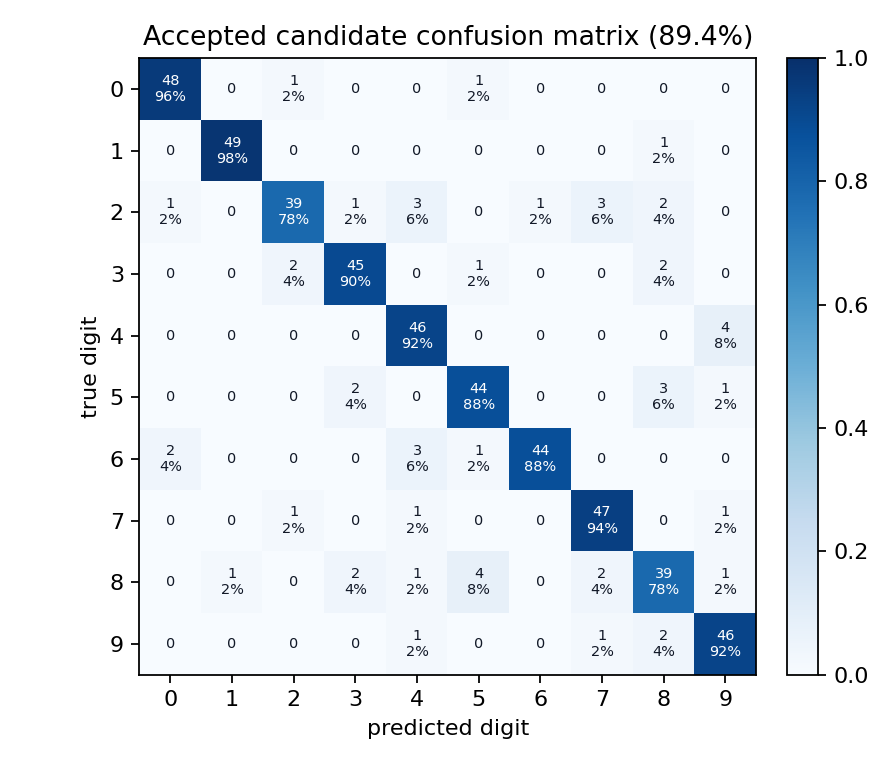
\includegraphics[keepaspectratio,alt={Accepted-candidate confusion matrix for exp-mlp-tanh-64 on the fixed MNIST handwritten digit database test split, sourced from output/data/ml\_confusion\_matrix.csv; it diagnoses the selected run, not general full-dataset performance. Generation method: Row-normalized heatmap with cell counts and row percentages. Registry metadata records the generation method, source artifact, and claim boundary for validation.}]{../figures/ml_confusion_matrix.png}}
\caption{Accepted-candidate confusion matrix for exp-mlp-tanh-64 on the
fixed MNIST handwritten digit database test split, sourced from
output/data/ml\_confusion\_matrix.csv; it diagnoses the selected run,
not general full-dataset performance. Generation method: Row-normalized
heatmap with cell counts and row percentages. Registry metadata records
the generation method, source artifact, and claim boundary for
validation.}\label{fig:ml_confusion_matrix}
\end{figure}

\begin{figure}
\centering
\pandocbounded{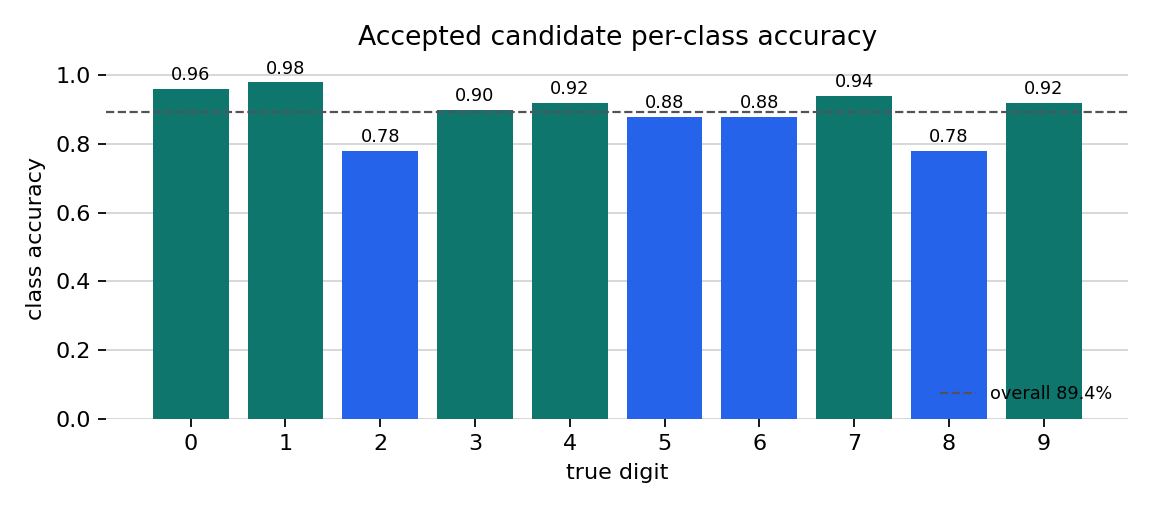
\includegraphics[keepaspectratio,alt={Per-class accuracy for exp-mlp-tanh-64, computed from output/data/ml\_confusion\_matrix.csv; variation across digits is a run diagnostic for the fixed local test split. Generation method: Per-class accuracy bars computed from the confusion matrix diagonal. Registry metadata records the generation method, source artifact, and claim boundary for validation.}]{../figures/ml_per_class_accuracy.png}}
\caption{Per-class accuracy for exp-mlp-tanh-64, computed from
output/data/ml\_confusion\_matrix.csv; variation across digits is a run
diagnostic for the fixed local test split. Generation method: Per-class
accuracy bars computed from the confusion matrix diagonal. Registry
metadata records the generation method, source artifact, and claim
boundary for validation.}\label{fig:ml_per_class_accuracy}
\end{figure}
\end{frame}

\begin{frame}[fragile,allowframebreaks]{Training And Error Diagnostics}
\protect\phantomsection\label{sec:training-error-diagnostics}
\begin{figure}
\centering
\pandocbounded{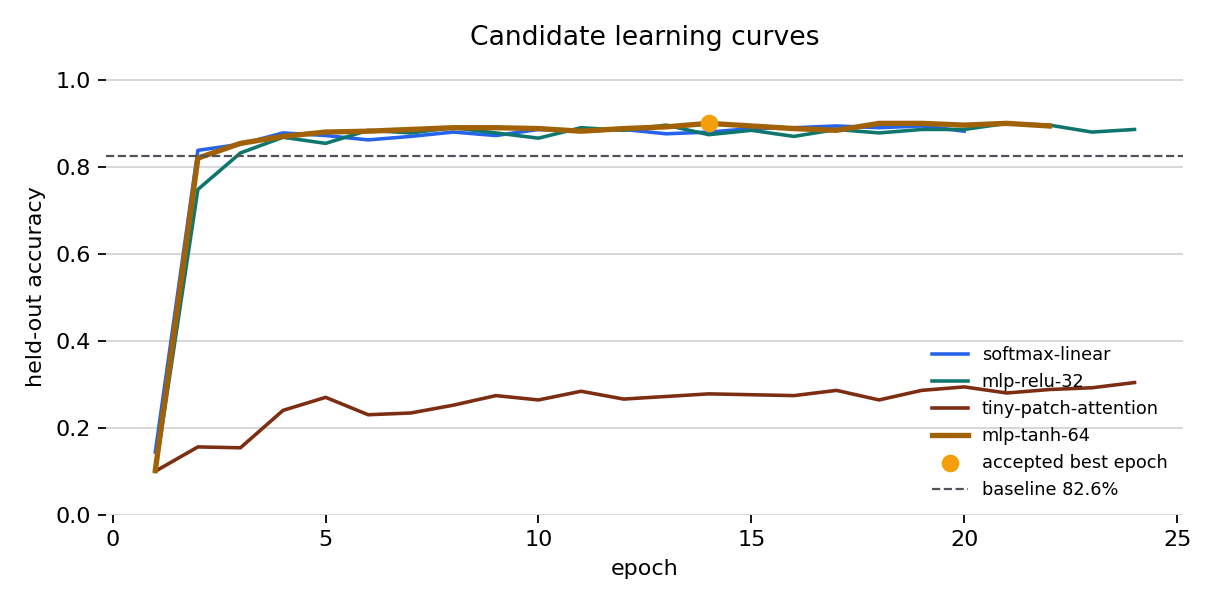
\includegraphics[keepaspectratio,alt={Epoch-level held-out accuracy curves for evaluated candidates from output/data/ml\_training\_history.csv; the accepted curve is visually emphasized for exp-mlp-tanh-64. Generation method: Epoch-level held-out accuracy lines with accepted best-epoch marker. Registry metadata records the generation method, source artifact, and claim boundary for validation.}]{../figures/ml_learning_curves.png}}
\caption{Epoch-level held-out accuracy curves for evaluated candidates
from output/data/ml\_training\_history.csv; the accepted curve is
visually emphasized for exp-mlp-tanh-64. Generation method: Epoch-level
held-out accuracy lines with accepted best-epoch marker. Registry
metadata records the generation method, source artifact, and claim
boundary for validation.}\label{fig:ml_learning_curves}
\end{figure}

\begin{figure}
\centering
\pandocbounded{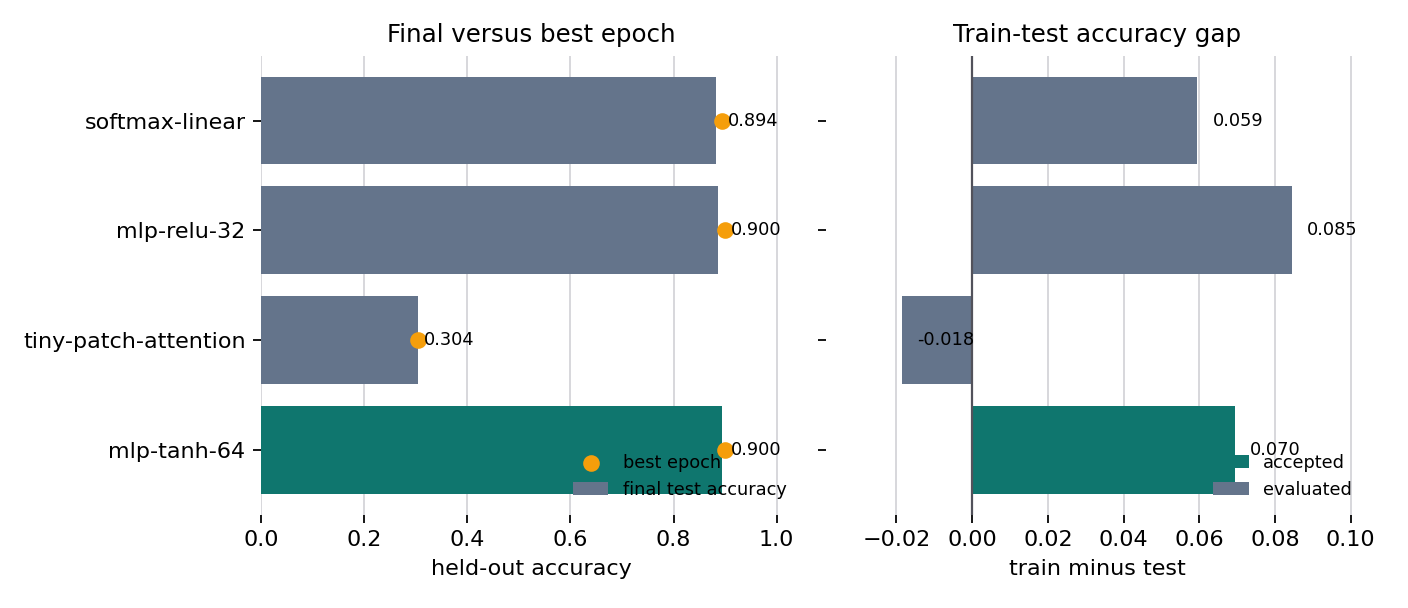
\includegraphics[keepaspectratio,alt={Configured-training dynamics for evaluated candidates from output/data/ml\_training\_diagnostics.json; exp-mlp-tanh-64 is highlighted while best-epoch markers and train-test gaps remain bounded to the local run. Generation method: Final and best-epoch accuracy bars plus train-test gap bars. Registry metadata records the generation method, source artifact, and claim boundary for validation.}]{../figures/ml_training_dynamics.png}}
\caption{Configured-training dynamics for evaluated candidates from
output/data/ml\_training\_diagnostics.json; exp-mlp-tanh-64 is
highlighted while best-epoch markers and train-test gaps remain bounded
to the local run. Generation method: Final and best-epoch accuracy bars
plus train-test gap bars. Registry metadata records the generation
method, source artifact, and claim boundary for
validation.}\label{fig:ml_training_dynamics}
\end{figure}

\begin{figure}
\centering
\pandocbounded{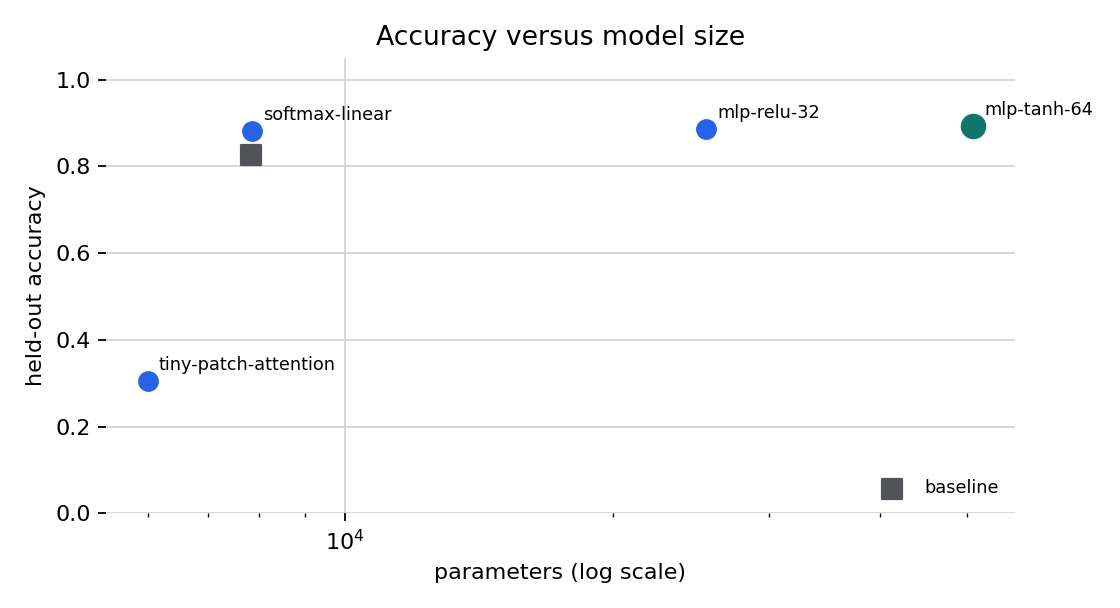
\includegraphics[keepaspectratio,alt={Parameter-count versus held-out accuracy for the baseline and evaluated candidates from output/data/ml\_task\_results.json; the accepted candidate is highlighted without claiming a general scaling law. Generation method: Log-parameter scatter plot against held-out accuracy. Registry metadata records the generation method, source artifact, and claim boundary for validation.}]{../figures/ml_complexity_accuracy.png}}
\caption{Parameter-count versus held-out accuracy for the baseline and
evaluated candidates from output/data/ml\_task\_results.json; the
accepted candidate is highlighted without claiming a general scaling
law. Generation method: Log-parameter scatter plot against held-out
accuracy. Registry metadata records the generation method, source
artifact, and claim boundary for
validation.}\label{fig:ml_complexity_accuracy}
\end{figure}

\begin{figure}
\centering
\pandocbounded{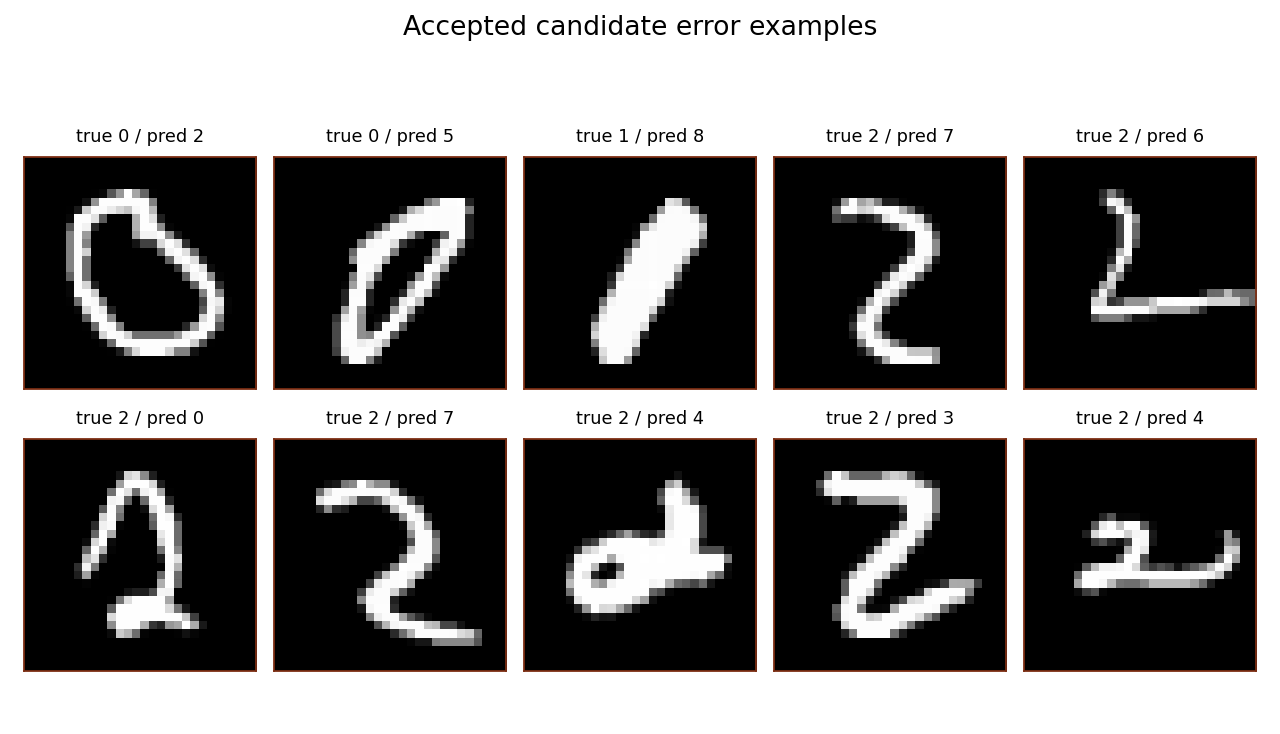
\includegraphics[keepaspectratio,alt={First accepted-candidate error examples for exp-mlp-tanh-64, sourced from output/data/ml\_error\_examples.json and data/mnist\_small.npz; these images support qualitative diagnosis only. Generation method: Deterministic grid of the first accepted-candidate misclassifications. Registry metadata records the generation method, source artifact, and claim boundary for validation.}]{../figures/mnist_error_examples.png}}
\caption{First accepted-candidate error examples for exp-mlp-tanh-64,
sourced from output/data/ml\_error\_examples.json and
data/mnist\_small.npz; these images support qualitative diagnosis only.
Generation method: Deterministic grid of the first accepted-candidate
misclassifications. Registry metadata records the generation method,
source artifact, and claim boundary for
validation.}\label{fig:mnist_error_examples}
\end{figure}

\begin{figure}
\centering
\pandocbounded{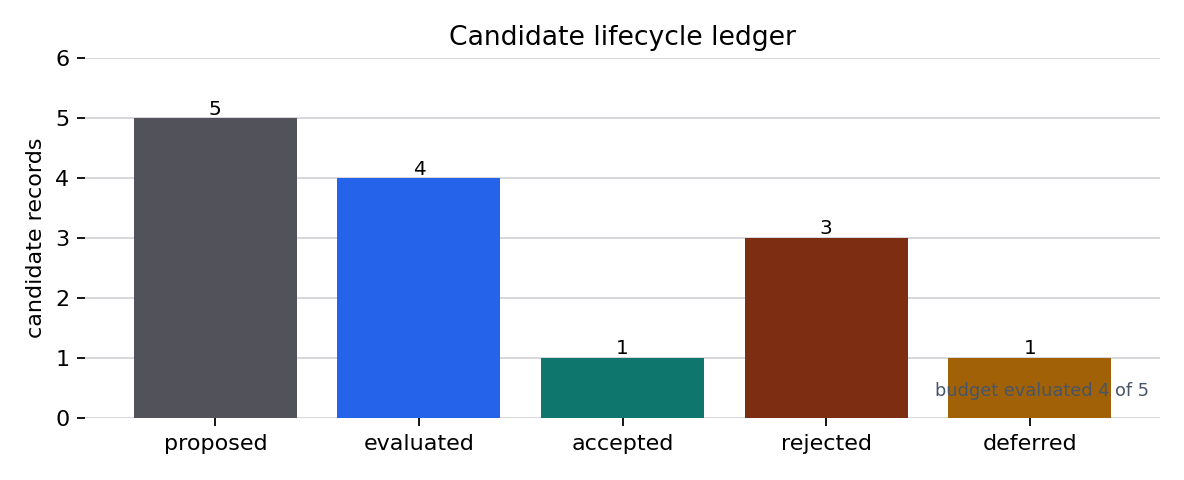
\includegraphics[keepaspectratio,alt={Candidate lifecycle ledger from output/data/ml\_candidate\_ledger.json: 4 evaluated out of 5 proposed candidates, with deferred proposals kept visible instead of executed automatically. Generation method: Candidate lifecycle status-count bar chart. Registry metadata records the generation method, source artifact, and claim boundary for validation.}]{../figures/autoresearch_candidate_lifecycle.png}}
\caption{Candidate lifecycle ledger from
output/data/ml\_candidate\_ledger.json: 4 evaluated out of 5 proposed
candidates, with deferred proposals kept visible instead of executed
automatically. Generation method: Candidate lifecycle status-count bar
chart. Registry metadata records the generation method, source artifact,
and claim boundary for
validation.}\label{fig:autoresearch_candidate_lifecycle}
\end{figure}

The selected candidate's best held-out epoch is \texttt{14}, its final
learning rate is \texttt{0.144}, its train-loss reduction is
\texttt{4.161}, and its final train-test accuracy gap is \texttt{7.0\%}.
These values come from the configured training diagnostics rather than
from a manually maintained result summary.

\begin{longtable}[]{@{}
  >{\raggedright\arraybackslash}p{(\linewidth - 14\tabcolsep) * \real{0.1250}}
  >{\raggedright\arraybackslash}p{(\linewidth - 14\tabcolsep) * \real{0.1250}}
  >{\raggedright\arraybackslash}p{(\linewidth - 14\tabcolsep) * \real{0.1250}}
  >{\raggedright\arraybackslash}p{(\linewidth - 14\tabcolsep) * \real{0.1250}}
  >{\raggedright\arraybackslash}p{(\linewidth - 14\tabcolsep) * \real{0.1250}}
  >{\raggedright\arraybackslash}p{(\linewidth - 14\tabcolsep) * \real{0.1250}}
  >{\raggedright\arraybackslash}p{(\linewidth - 14\tabcolsep) * \real{0.1250}}
  >{\raggedright\arraybackslash}p{(\linewidth - 14\tabcolsep) * \real{0.1250}}@{}}
\caption{Configured-training diagnostics from
\protect\breaktt{output/data/ml\_training\_diagnostics.json}.}\label{tbl:training-diagnostics}\tabularnewline
\toprule\noalign{}
\begin{minipage}[b]{\linewidth}\raggedright
Candidate
\end{minipage} & \begin{minipage}[b]{\linewidth}\raggedright
Status
\end{minipage} & \begin{minipage}[b]{\linewidth}\raggedright
Best epoch
\end{minipage} & \begin{minipage}[b]{\linewidth}\raggedright
Best test accuracy
\end{minipage} & \begin{minipage}[b]{\linewidth}\raggedright
Final test accuracy
\end{minipage} & \begin{minipage}[b]{\linewidth}\raggedright
Train-test gap
\end{minipage} & \begin{minipage}[b]{\linewidth}\raggedright
Loss reduction
\end{minipage} & \begin{minipage}[b]{\linewidth}\raggedright
Final learning rate
\end{minipage} \\
\midrule\noalign{}
\endfirsthead
\toprule\noalign{}
\begin{minipage}[b]{\linewidth}\raggedright
Candidate
\end{minipage} & \begin{minipage}[b]{\linewidth}\raggedright
Status
\end{minipage} & \begin{minipage}[b]{\linewidth}\raggedright
Best epoch
\end{minipage} & \begin{minipage}[b]{\linewidth}\raggedright
Best test accuracy
\end{minipage} & \begin{minipage}[b]{\linewidth}\raggedright
Final test accuracy
\end{minipage} & \begin{minipage}[b]{\linewidth}\raggedright
Train-test gap
\end{minipage} & \begin{minipage}[b]{\linewidth}\raggedright
Loss reduction
\end{minipage} & \begin{minipage}[b]{\linewidth}\raggedright
Final learning rate
\end{minipage} \\
\midrule\noalign{}
\endhead
softmax linear & rejected & 17 & 89.4\% & 88.2\% & 5.9\% & 2.917 &
0.273 \\
mlp relu 32 & rejected & 21 & 90.0\% & 88.6\% & 8.5\% & 4.341 & 0.178 \\
tiny patch attention & rejected & 24 & 30.4\% & 30.4\% & -1.8\% & 0.165
& 0.214 \\
mlp tanh 64 & accepted & 14 & 90.0\% & 89.4\% & 7.0\% & 4.161 & 0.144 \\
\bottomrule\noalign{}
\end{longtable}
\end{frame}

\begin{frame}[fragile,allowframebreaks]{Diagnostic Analysis}
\protect\phantomsection\label{sec:diagnostic-analysis}
The selected candidate macro F1 is \texttt{89.4\%}, with a held-out
accuracy interval of \breaktt{86.4\%\ to\ 91.8\%}. Probability
diagnostics report expected calibration error \texttt{2.9\%} and
\texttt{11} high-confidence error(s). The top non-diagonal confusion
pair is \texttt{4\ -\textgreater{}\ 9\ (4)}, and the minimum
selected-candidate accuracy across deterministic robustness transforms
is \texttt{80.0\%}. These values are descriptive diagnostics for the
validated local run, not external benchmark claims.

\begin{block}{Classification And Error Structure}
\protect\phantomsection\label{sec:classification-error-structure}
The class-level and error-pattern diagnostics are intentionally
visual-first: @fig:ml\_calibration\_reliability checks confidence
calibration, @fig:ml\_classification\_metrics\_heatmap separates
precision, recall, and F1 by digit, and @fig:ml\_confusion\_pairs ranks
the non-diagonal confusions that most shape the selected-candidate error
profile. The accompanying tables preserve the same values for audit and
downstream comparison.

\begin{figure}
\centering
\pandocbounded{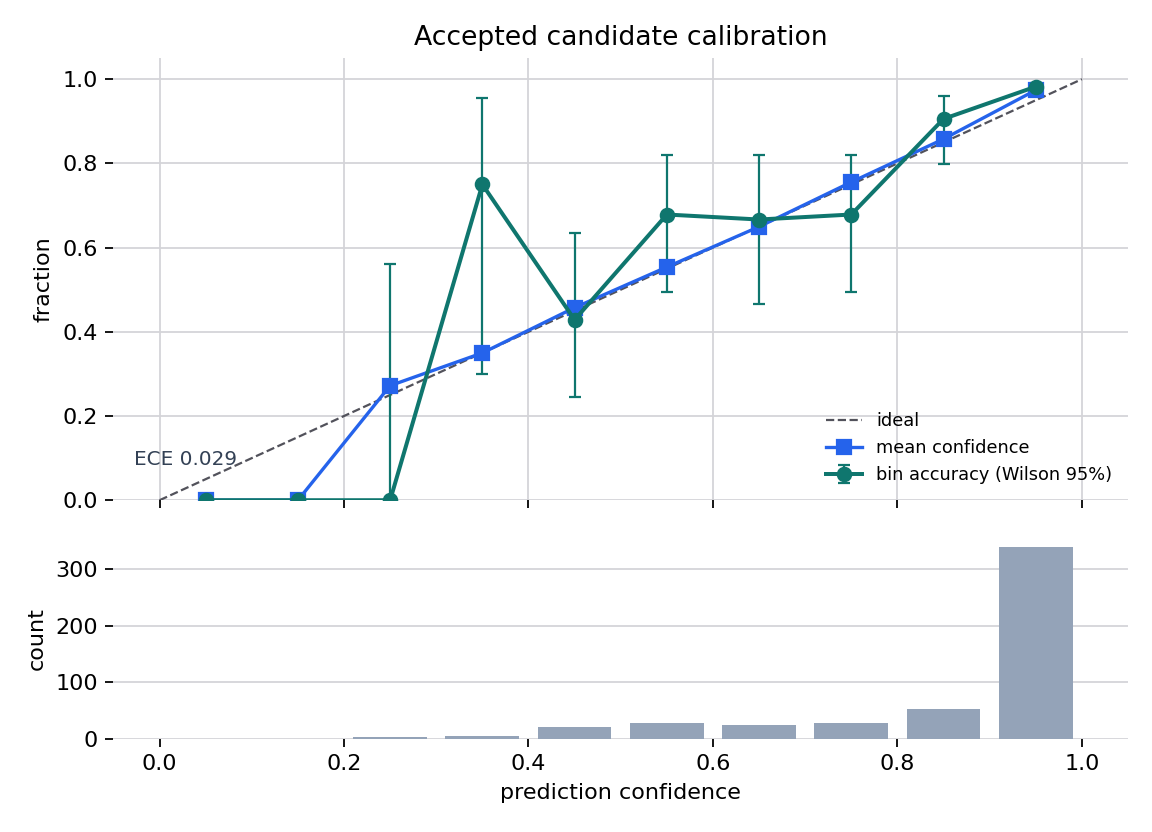
\includegraphics[keepaspectratio,alt={Reliability curve for exp-mlp-tanh-64 from output/data/ml\_calibration\_report.json; expected calibration error and bin counts summarize the accepted candidate on the fixed local test split. Generation method: Reliability curve with confidence-bin support histogram. Registry metadata records the generation method, source artifact, and claim boundary for validation.}]{../figures/ml_calibration_reliability.png}}
\caption{Reliability curve for exp-mlp-tanh-64 from
output/data/ml\_calibration\_report.json; expected calibration error and
bin counts summarize the accepted candidate on the fixed local test
split. Generation method: Reliability curve with confidence-bin support
histogram. Registry metadata records the generation method, source
artifact, and claim boundary for
validation.}\label{fig:ml_calibration_reliability}
\end{figure}

\begin{figure}
\centering
\pandocbounded{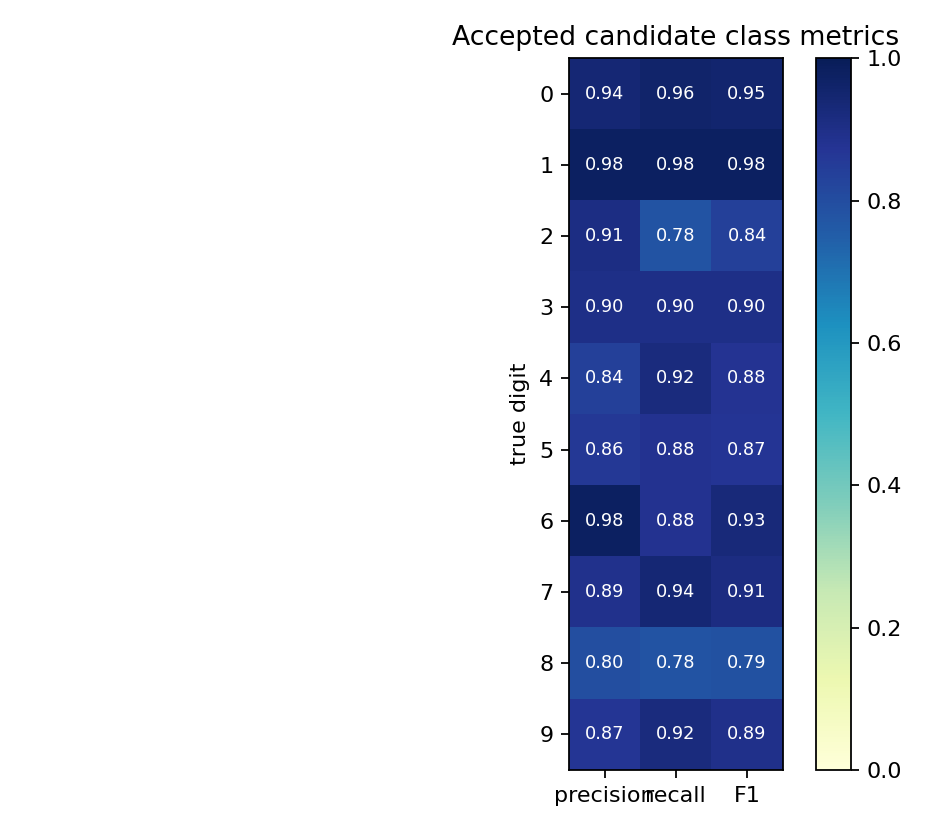
\includegraphics[keepaspectratio,alt={Per-class precision, recall, and F1 for exp-mlp-tanh-64, sourced from output/data/ml\_classification\_diagnostics.json; metrics are scoped to the local test split. Generation method: Per-class precision, recall, and F1 heatmap. Registry metadata records the generation method, source artifact, and claim boundary for validation.}]{../figures/ml_classification_metrics_heatmap.png}}
\caption{Per-class precision, recall, and F1 for exp-mlp-tanh-64,
sourced from output/data/ml\_classification\_diagnostics.json; metrics
are scoped to the local test split. Generation method: Per-class
precision, recall, and F1 heatmap. Registry metadata records the
generation method, source artifact, and claim boundary for
validation.}\label{fig:ml_classification_metrics_heatmap}
\end{figure}

\begin{figure}
\centering
\pandocbounded{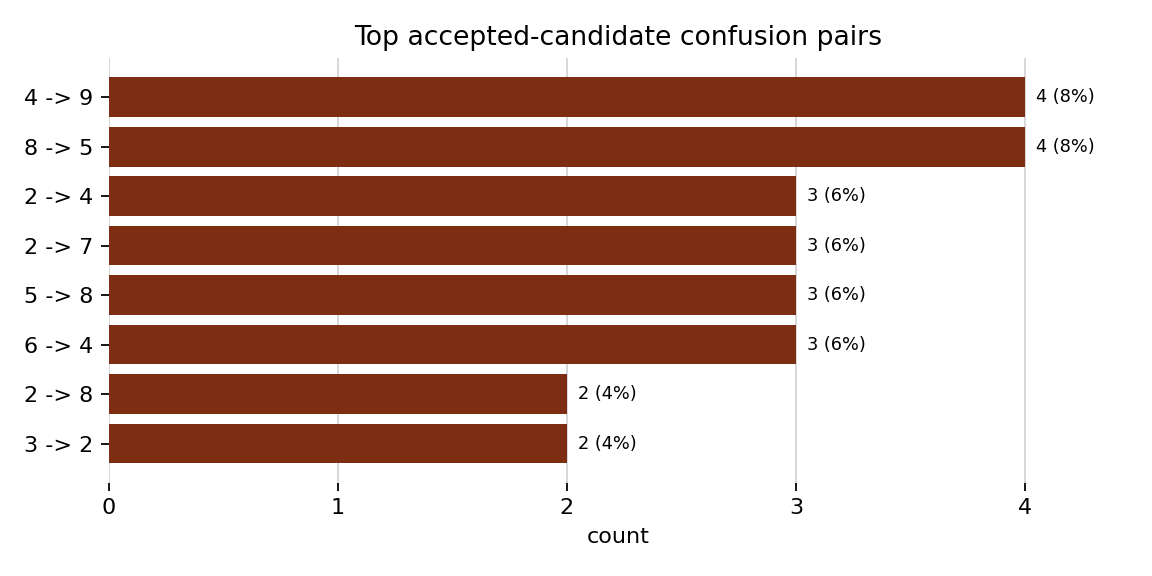
\includegraphics[keepaspectratio,alt={Top non-diagonal confusion pairs for exp-mlp-tanh-64, sourced from output/data/ml\_classification\_diagnostics.json; the bars highlight which local digit pairs account for accepted-candidate errors. Generation method: Ranked off-diagonal confusion-pair bars with true-class error rates. Registry metadata records the generation method, source artifact, and claim boundary for validation.}]{../figures/ml_confusion_pairs.png}}
\caption{Top non-diagonal confusion pairs for exp-mlp-tanh-64, sourced
from output/data/ml\_classification\_diagnostics.json; the bars
highlight which local digit pairs account for accepted-candidate errors.
Generation method: Ranked off-diagonal confusion-pair bars with
true-class error rates. Registry metadata records the generation method,
source artifact, and claim boundary for
validation.}\label{fig:ml_confusion_pairs}
\end{figure}

\begin{longtable}[]{@{}lllll@{}}
\caption{Accepted-candidate class diagnostics from
\protect\breaktt{output/data/ml\_classification\_diagnostics.json}.}\label{tbl:classification-diagnostics}\tabularnewline
\toprule\noalign{}
Class & Precision & Recall & F1 & Support \\
\midrule\noalign{}
\endfirsthead
\toprule\noalign{}
Class & Precision & Recall & F1 & Support \\
\midrule\noalign{}
\endhead
0 & 94.1\% & 96.0\% & 95.0\% & 50 \\
1 & 98.0\% & 98.0\% & 98.0\% & 50 \\
2 & 90.7\% & 78.0\% & 83.9\% & 50 \\
3 & 90.0\% & 90.0\% & 90.0\% & 50 \\
4 & 83.6\% & 92.0\% & 87.6\% & 50 \\
5 & 86.3\% & 88.0\% & 87.1\% & 50 \\
6 & 97.8\% & 88.0\% & 92.6\% & 50 \\
7 & 88.7\% & 94.0\% & 91.3\% & 50 \\
8 & 79.6\% & 78.0\% & 78.8\% & 50 \\
9 & 86.8\% & 92.0\% & 89.3\% & 50 \\
\bottomrule\noalign{}
\end{longtable}

\begin{longtable}[]{@{}lllll@{}}
\caption{Calibration bins from
\protect\breaktt{output/data/ml\_calibration\_report.json}.}\label{tbl:calibration-bins}\tabularnewline
\toprule\noalign{}
Confidence bin & Count & Accuracy & Mean confidence & Gap \\
\midrule\noalign{}
\endfirsthead
\toprule\noalign{}
Confidence bin & Count & Accuracy & Mean confidence & Gap \\
\midrule\noalign{}
\endhead
0-0.1 & 0 & 0.0\% & 0.0\% & 0.0\% \\
0.1-0.2 & 0 & 0.0\% & 0.0\% & 0.0\% \\
0.2-0.3 & 3 & 0.0\% & 27.2\% & 27.2\% \\
0.3-0.4 & 4 & 75.0\% & 35.0\% & 40.0\% \\
0.4-0.5 & 21 & 42.9\% & 45.7\% & 2.9\% \\
0.5-0.6 & 28 & 67.9\% & 55.4\% & 12.5\% \\
0.6-0.7 & 24 & 66.7\% & 65.0\% & 1.7\% \\
0.7-0.8 & 28 & 67.9\% & 75.6\% & 7.7\% \\
0.8-0.9 & 53 & 90.6\% & 85.8\% & 4.8\% \\
0.9-1 & 339 & 98.2\% & 97.4\% & 0.8\% \\
\bottomrule\noalign{}
\end{longtable}

\begin{longtable}[]{@{}llllll@{}}
\caption{Calibration-bin Wilson intervals from
\protect\breaktt{output/data/ml\_calibration\_bin\_intervals.json}; empty
bins are reported
explicitly.}\label{tbl:calibration-bin-intervals}\tabularnewline
\toprule\noalign{}
Confidence bin & Count & Correct & Accuracy & Wilson 95\% & Empty \\
\midrule\noalign{}
\endfirsthead
\toprule\noalign{}
Confidence bin & Count & Correct & Accuracy & Wilson 95\% & Empty \\
\midrule\noalign{}
\endhead
0-0.1 & 0 & 0 & 0.0\% & 0.0\% to 0.0\% & True \\
0.1-0.2 & 0 & 0 & 0.0\% & 0.0\% to 0.0\% & True \\
0.2-0.3 & 3 & 0 & 0.0\% & 0.0\% to 56.2\% & False \\
0.3-0.4 & 4 & 3 & 75.0\% & 30.1\% to 95.4\% & False \\
0.4-0.5 & 21 & 9 & 42.9\% & 24.5\% to 63.5\% & False \\
0.5-0.6 & 28 & 19 & 67.9\% & 49.3\% to 82.1\% & False \\
0.6-0.7 & 24 & 16 & 66.7\% & 46.7\% to 82.0\% & False \\
0.7-0.8 & 28 & 19 & 67.9\% & 49.3\% to 82.1\% & False \\
0.8-0.9 & 53 & 48 & 90.6\% & 79.7\% to 95.9\% & False \\
0.9-1 & 339 & 333 & 98.2\% & 96.2\% to 99.2\% & False \\
\bottomrule\noalign{}
\end{longtable}

\begin{longtable}[]{@{}lll@{}}
\caption{Top non-diagonal confusion pairs from
\protect\breaktt{output/data/ml\_classification\_diagnostics.json}.}\label{tbl:confusion-pairs}\tabularnewline
\toprule\noalign{}
Pair & Count & True-class error rate \\
\midrule\noalign{}
\endfirsthead
\toprule\noalign{}
Pair & Count & True-class error rate \\
\midrule\noalign{}
\endhead
4 -\textgreater{} 9 & 4 & 8.0\% \\
8 -\textgreater{} 5 & 4 & 8.0\% \\
2 -\textgreater{} 4 & 3 & 6.0\% \\
2 -\textgreater{} 7 & 3 & 6.0\% \\
5 -\textgreater{} 8 & 3 & 6.0\% \\
6 -\textgreater{} 4 & 3 & 6.0\% \\
2 -\textgreater{} 8 & 2 & 4.0\% \\
3 -\textgreater{} 2 & 2 & 4.0\% \\
3 -\textgreater{} 8 & 2 & 4.0\% \\
5 -\textgreater{} 3 & 2 & 4.0\% \\
\bottomrule\noalign{}
\end{longtable}
\end{block}

\begin{block}{Uncertainty, Generalization, And Perturbation}
\protect\phantomsection\label{sec:uncertainty-generalization-perturbation}
Additional uncertainty and matched-comparison diagnostics report
bootstrap accuracy interval \breaktt{86.4\%\ to\ 92.0\%}, bootstrap
macro-F1 interval \breaktt{86.5\%\ to\ 91.9\%}, paired net accuracy gain
\texttt{6.8\%}, exact McNemar p-value \texttt{0.000}, mean
correct-prediction confidence \texttt{90.9\%}, mean error confidence
\texttt{63.1\%}, and \texttt{22} low-margin selected-candidate
prediction(s). These diagnostics are generated from the fixed local test
split and are reported as run evidence, not as population-level
certification.

@fig:ml\_generalization\_gap compares train and test behavior,
@fig:ml\_robustness\_matrix shows deterministic no-retrain perturbation
results, @fig:ml\_probability\_margin\_distribution summarizes
confidence and margin distributions, @fig:ml\_bootstrap\_intervals shows
local resampling intervals, and @fig:ml\_paired\_correctness exposes the
matched selected-versus-baseline correctness table used by the paired
comparison.

\begin{figure}
\centering
\pandocbounded{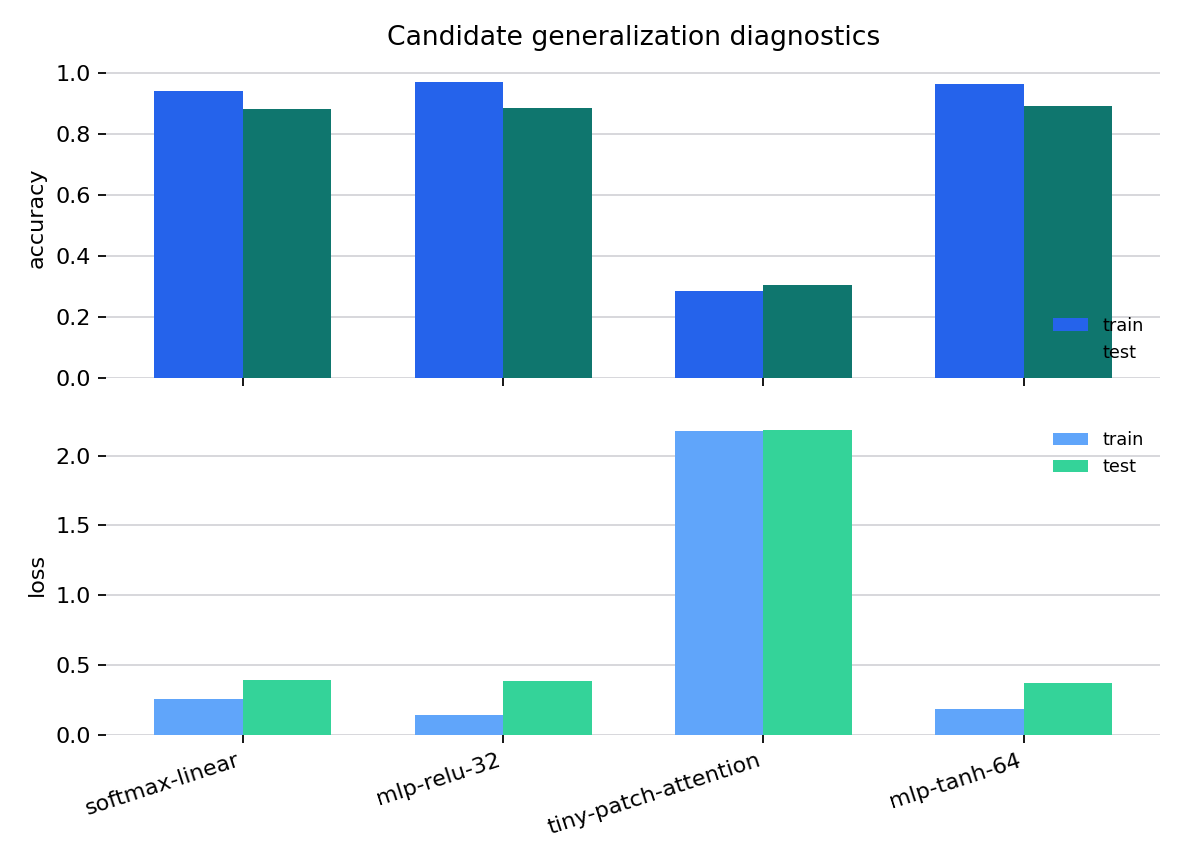
\includegraphics[keepaspectratio,alt={Train/test accuracy and loss for evaluated candidates from output/data/ml\_classification\_diagnostics.json; the plot exposes local generalization gaps without claiming full-dataset behavior. Generation method: Grouped train/test accuracy and loss bars by evaluated candidate. Registry metadata records the generation method, source artifact, and claim boundary for validation.}]{../figures/ml_generalization_gap.png}}
\caption{Train/test accuracy and loss for evaluated candidates from
output/data/ml\_classification\_diagnostics.json; the plot exposes local
generalization gaps without claiming full-dataset behavior. Generation
method: Grouped train/test accuracy and loss bars by evaluated
candidate. Registry metadata records the generation method, source
artifact, and claim boundary for
validation.}\label{fig:ml_generalization_gap}
\end{figure}

\begin{figure}
\centering
\pandocbounded{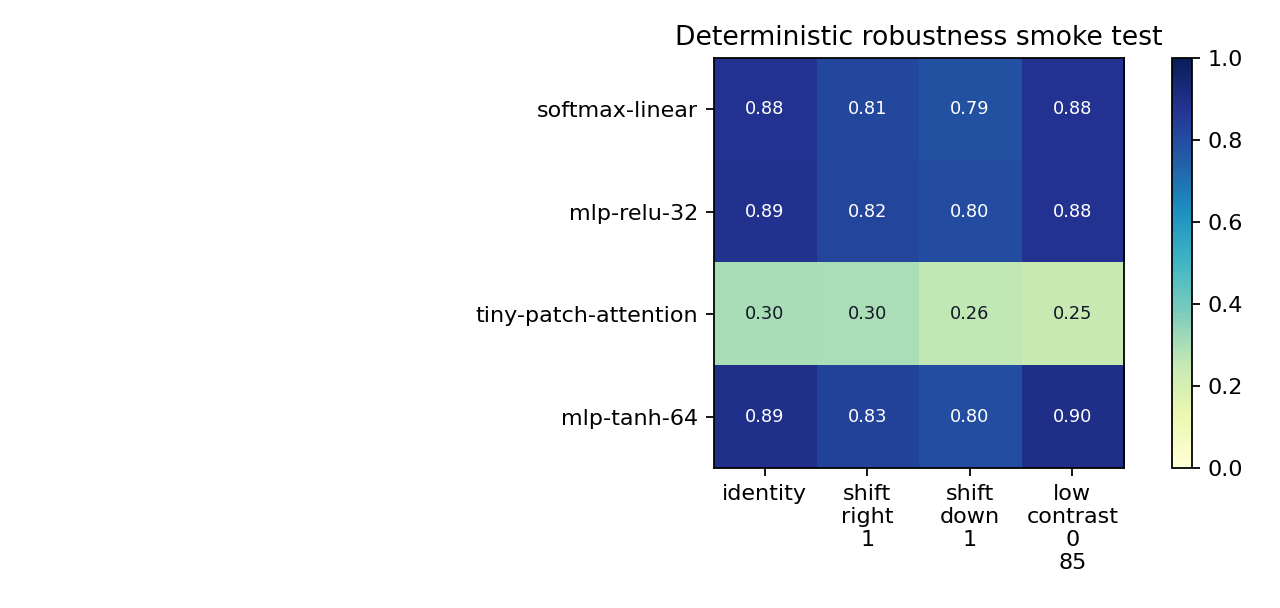
\includegraphics[keepaspectratio,alt={Accuracy for evaluated candidates under identity, one-pixel shifts, and low contrast from output/data/ml\_robustness\_report.json; the deterministic transforms provide a bounded smoke test only. Generation method: Candidate-by-transform accuracy heatmap for deterministic perturbations. Registry metadata records the generation method, source artifact, and claim boundary for validation.}]{../figures/ml_robustness_matrix.png}}
\caption{Accuracy for evaluated candidates under identity, one-pixel
shifts, and low contrast from output/data/ml\_robustness\_report.json;
the deterministic transforms provide a bounded smoke test only.
Generation method: Candidate-by-transform accuracy heatmap for
deterministic perturbations. Registry metadata records the generation
method, source artifact, and claim boundary for
validation.}\label{fig:ml_robustness_matrix}
\end{figure}

\begin{figure}
\centering
\pandocbounded{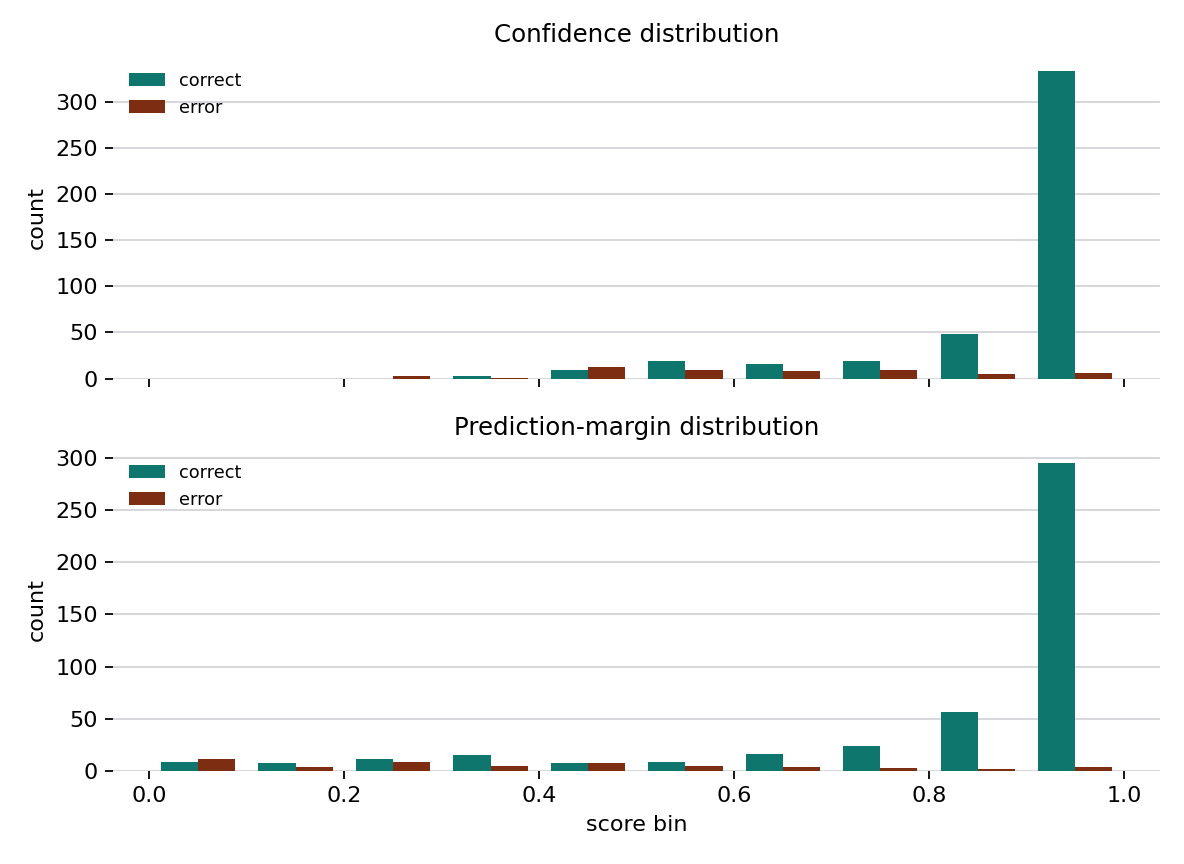
\includegraphics[keepaspectratio,alt={Confidence and prediction-margin histograms for exp-mlp-tanh-64 from output/data/ml\_probability\_diagnostics.json; the figure separates correct and incorrect local test predictions. Generation method: Confidence and margin histograms split by correctness. Registry metadata records the generation method, source artifact, and claim boundary for validation.}]{../figures/ml_probability_margin_distribution.png}}
\caption{Confidence and prediction-margin histograms for exp-mlp-tanh-64
from output/data/ml\_probability\_diagnostics.json; the figure separates
correct and incorrect local test predictions. Generation method:
Confidence and margin histograms split by correctness. Registry metadata
records the generation method, source artifact, and claim boundary for
validation.}\label{fig:ml_probability_margin_distribution}
\end{figure}

\begin{figure}
\centering
\pandocbounded{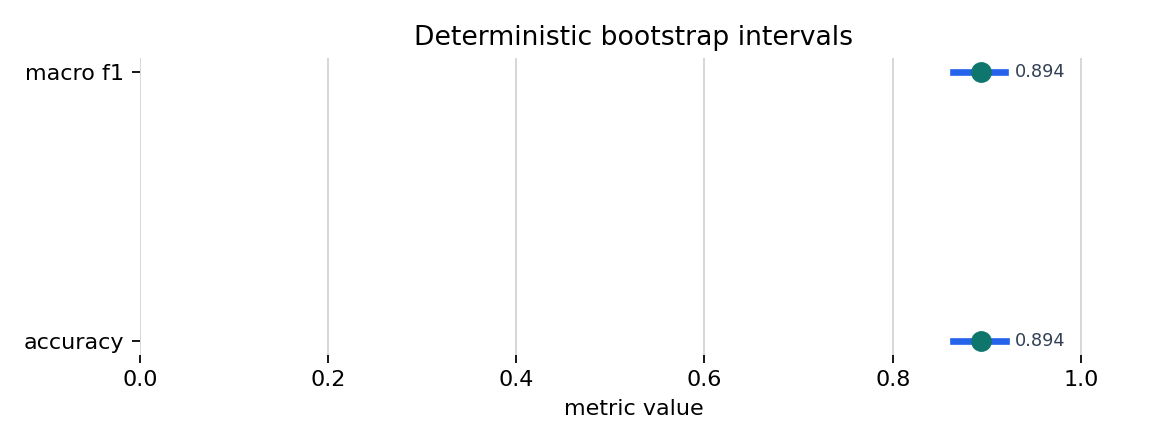
\includegraphics[keepaspectratio,alt={Deterministic percentile-bootstrap intervals for exp-mlp-tanh-64 from output/data/ml\_bootstrap\_intervals.json; the intervals summarize local sampling variation for accuracy and macro F1. Generation method: Horizontal percentile-bootstrap interval plot. Registry metadata records the generation method, source artifact, and claim boundary for validation.}]{../figures/ml_bootstrap_intervals.png}}
\caption{Deterministic percentile-bootstrap intervals for
exp-mlp-tanh-64 from output/data/ml\_bootstrap\_intervals.json; the
intervals summarize local sampling variation for accuracy and macro F1.
Generation method: Horizontal percentile-bootstrap interval plot.
Registry metadata records the generation method, source artifact, and
claim boundary for validation.}\label{fig:ml_bootstrap_intervals}
\end{figure}

\begin{figure}
\centering
\pandocbounded{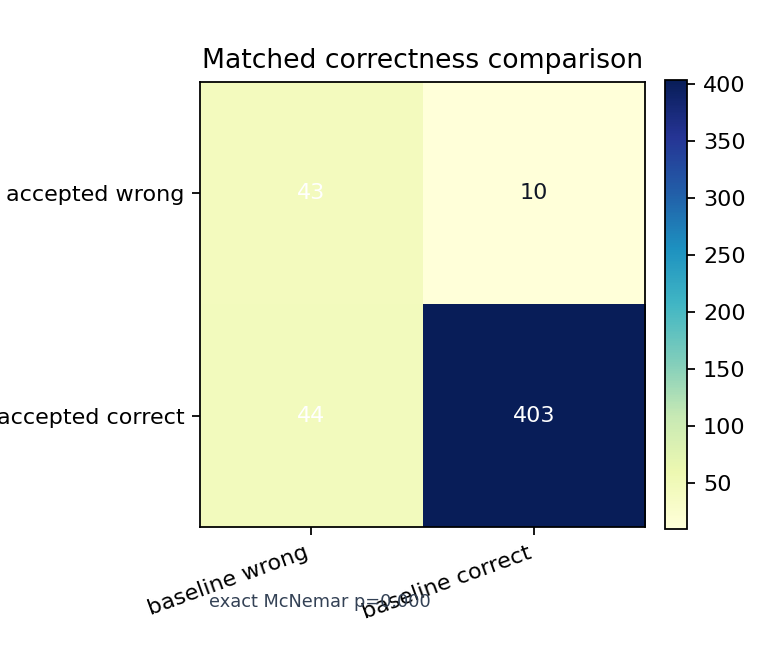
\includegraphics[keepaspectratio,alt={Matched correctness comparison between exp-mlp-tanh-64 and the nearest\_centroid\_baseline baseline from output/data/ml\_paired\_comparison.json; discordant cells support the paired test summary. Generation method: Matched accepted-versus-baseline correctness heatmap. Registry metadata records the generation method, source artifact, and claim boundary for validation.}]{../figures/ml_paired_correctness.png}}
\caption{Matched correctness comparison between exp-mlp-tanh-64 and the
nearest\_centroid\_baseline baseline from
output/data/ml\_paired\_comparison.json; discordant cells support the
paired test summary. Generation method: Matched accepted-versus-baseline
correctness heatmap. Registry metadata records the generation method,
source artifact, and claim boundary for
validation.}\label{fig:ml_paired_correctness}
\end{figure}

\begin{longtable}[]{@{}llll@{}}
\caption{Deterministic no-retrain robustness smoke test from
\protect\breaktt{output/data/ml\_robustness\_report.json}.}\label{tbl:robustness-scores}\tabularnewline
\toprule\noalign{}
Candidate & Transform & Accuracy & Samples \\
\midrule\noalign{}
\endfirsthead
\toprule\noalign{}
Candidate & Transform & Accuracy & Samples \\
\midrule\noalign{}
\endhead
softmax linear & identity & 88.2\% & 500 \\
softmax linear & shift\_right\_1 & 81.4\% & 500 \\
softmax linear & shift\_down\_1 & 78.6\% & 500 \\
softmax linear & low\_contrast\_0\_85 & 88.0\% & 500 \\
mlp relu 32 & identity & 88.6\% & 500 \\
mlp relu 32 & shift\_right\_1 & 82.4\% & 500 \\
mlp relu 32 & shift\_down\_1 & 80.2\% & 500 \\
mlp relu 32 & low\_contrast\_0\_85 & 88.2\% & 500 \\
tiny patch attention & identity & 30.4\% & 500 \\
tiny patch attention & shift\_right\_1 & 29.8\% & 500 \\
tiny patch attention & shift\_down\_1 & 25.8\% & 500 \\
tiny patch attention & low\_contrast\_0\_85 & 24.6\% & 500 \\
mlp tanh 64 & identity & 89.4\% & 500 \\
mlp tanh 64 & shift\_right\_1 & 83.2\% & 500 \\
mlp tanh 64 & shift\_down\_1 & 80.0\% & 500 \\
mlp tanh 64 & low\_contrast\_0\_85 & 89.8\% & 500 \\
\bottomrule\noalign{}
\end{longtable}

\begin{longtable}[]{@{}ll@{}}
\caption{Accepted-candidate probability diagnostics from
\protect\breaktt{output/data/ml\_probability\_diagnostics.json}.}\label{tbl:probability-diagnostics}\tabularnewline
\toprule\noalign{}
Statistic & Value \\
\midrule\noalign{}
\endfirsthead
\toprule\noalign{}
Statistic & Value \\
\midrule\noalign{}
\endhead
Mean confidence & 87.9\% \\
Mean correct confidence & 90.9\% \\
Mean error confidence & 63.1\% \\
Mean margin & 80.2\% \\
Mean correct margin & 84.9\% \\
Mean error margin & 40.3\% \\
Low-margin count & 22 \\
\bottomrule\noalign{}
\end{longtable}

\begin{longtable}[]{@{}lllll@{}}
\caption{Deterministic percentile-bootstrap intervals from
\protect\breaktt{output/data/ml\_bootstrap\_intervals.json}.}\label{tbl:bootstrap-intervals}\tabularnewline
\toprule\noalign{}
Metric & Observed & CI low & CI high & Resample mean \\
\midrule\noalign{}
\endfirsthead
\toprule\noalign{}
Metric & Observed & CI low & CI high & Resample mean \\
\midrule\noalign{}
\endhead
accuracy & 89.4\% & 86.4\% & 92.0\% & 89.4\% \\
macro F1 & 89.4\% & 86.5\% & 91.9\% & 89.3\% \\
\bottomrule\noalign{}
\end{longtable}

\begin{longtable}[]{@{}ll@{}}
\caption{Accepted-candidate versus baseline paired comparison from
\protect\breaktt{output/data/ml\_paired\_comparison.json}.}\label{tbl:paired-comparison}\tabularnewline
\toprule\noalign{}
Matched comparison statistic & Value \\
\midrule\noalign{}
\endfirsthead
\toprule\noalign{}
Matched comparison statistic & Value \\
\midrule\noalign{}
\endhead
Both correct & 403 \\
Accepted only correct & 44 \\
Baseline only correct & 10 \\
Both wrong & 43 \\
Discordant examples & 54 \\
Exact McNemar p & 0.000 \\
Net accuracy gain & 6.8\% \\
\bottomrule\noalign{}
\end{longtable}
\end{block}

\begin{block}{Probability Quality And Selective Prediction}
\protect\phantomsection\label{sec:probability-quality-selective-prediction}
Probability-quality diagnostics report Brier score \texttt{0.161},
negative log likelihood \texttt{0.361}, top-2 accuracy \texttt{95.6\%},
and Cohen kappa \texttt{0.882} for the selected candidate. At the
highest configured confidence threshold, retained coverage is
\texttt{67.8\%} and selective accuracy is \texttt{98.2\%}.

The selective-prediction view in @fig:ml\_selective\_accuracy reports
the configured confidence-threshold trade-off: retaining fewer
predictions can raise selective accuracy, but the coverage table keeps
that trade-off explicit. The candidate probability-quality comparison in
@fig:ml\_probability\_quality keeps accuracy separate from proper-score
behavior, so the selected candidate is not treated as automatically best
on every diagnostic axis.

\begin{figure}
\centering
\pandocbounded{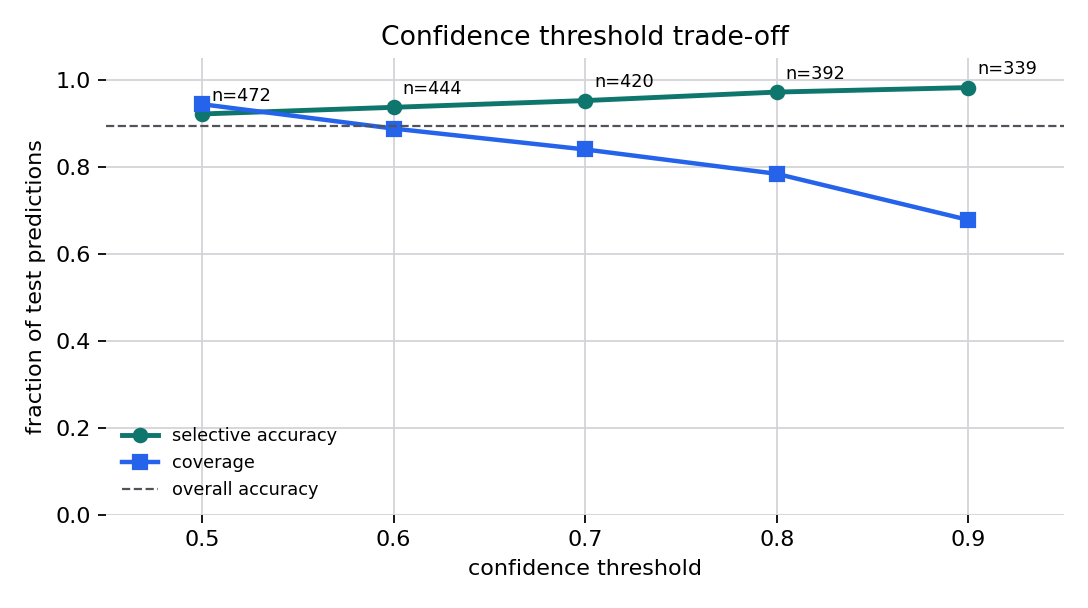
\includegraphics[keepaspectratio,alt={Confidence-threshold trade-off for exp-mlp-tanh-64 from output/data/ml\_statistical\_summary.json; the plot compares retained coverage, selective accuracy, and the unthresholded accepted-candidate accuracy on the fixed local split. Generation method: Confidence-threshold coverage and selective-accuracy line chart. Registry metadata records the generation method, source artifact, and claim boundary for validation.}]{../figures/ml_selective_accuracy.png}}
\caption{Confidence-threshold trade-off for exp-mlp-tanh-64 from
output/data/ml\_statistical\_summary.json; the plot compares retained
coverage, selective accuracy, and the unthresholded accepted-candidate
accuracy on the fixed local split. Generation method:
Confidence-threshold coverage and selective-accuracy line chart.
Registry metadata records the generation method, source artifact, and
claim boundary for validation.}\label{fig:ml_selective_accuracy}
\end{figure}

\begin{figure}
\centering
\pandocbounded{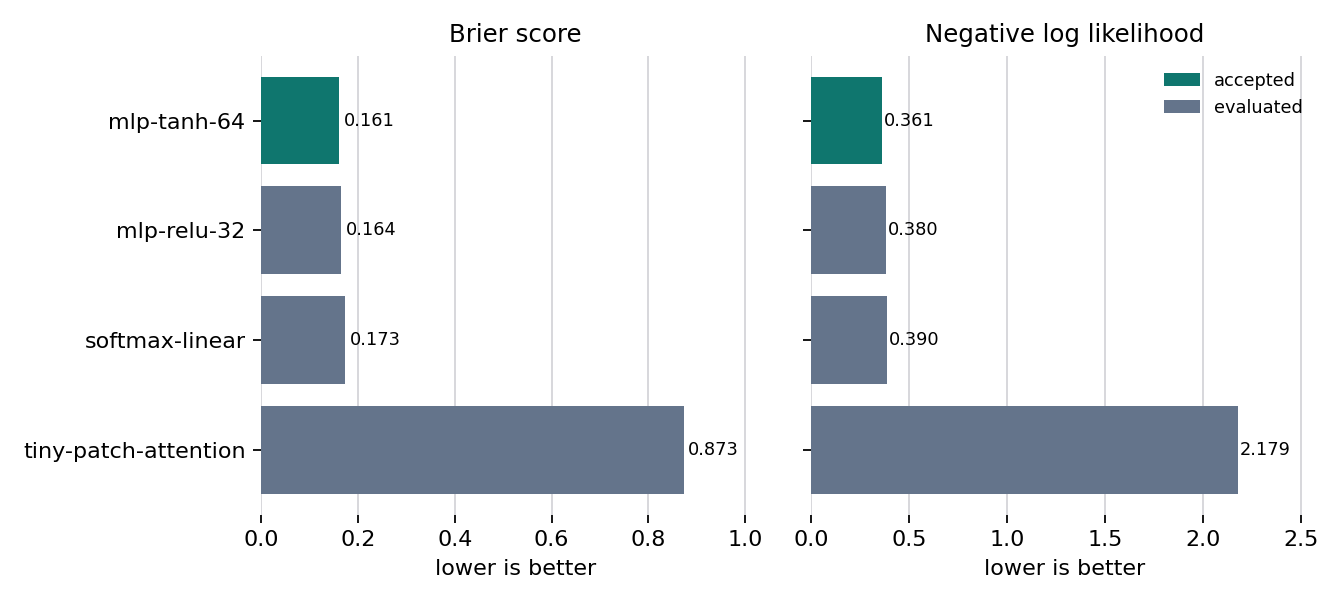
\includegraphics[keepaspectratio,alt={Brier score and negative log likelihood for evaluated candidates from output/data/ml\_statistical\_summary.json; lower values indicate better probability quality within the configured local run, and the accepted candidate is highlighted. Generation method: Brier score and negative-log-likelihood bar comparison. Registry metadata records the generation method, source artifact, and claim boundary for validation.}]{../figures/ml_probability_quality.png}}
\caption{Brier score and negative log likelihood for evaluated
candidates from output/data/ml\_statistical\_summary.json; lower values
indicate better probability quality within the configured local run, and
the accepted candidate is highlighted. Generation method: Brier score
and negative-log-likelihood bar comparison. Registry metadata records
the generation method, source artifact, and claim boundary for
validation.}\label{fig:ml_probability_quality}
\end{figure}

\begin{longtable}[]{@{}ll@{}}
\caption{Accepted-candidate statistical summary from
\protect\breaktt{output/data/ml\_statistical\_summary.json}.}\label{tbl:statistical-summary}\tabularnewline
\toprule\noalign{}
Statistic & Value \\
\midrule\noalign{}
\endfirsthead
\toprule\noalign{}
Statistic & Value \\
\midrule\noalign{}
\endhead
Accuracy & 89.4\% \\
Balanced accuracy & 89.4\% \\
Macro F1 & 89.4\% \\
Top-2 accuracy & 95.6\% \\
Cohen kappa & 0.882 \\
Brier score & 0.161 \\
Negative log likelihood & 0.361 \\
Expected calibration error & 2.9\% \\
\bottomrule\noalign{}
\end{longtable}

\begin{longtable}[]{@{}
  >{\raggedright\arraybackslash}p{(\linewidth - 8\tabcolsep) * \real{0.2000}}
  >{\raggedright\arraybackslash}p{(\linewidth - 8\tabcolsep) * \real{0.2000}}
  >{\raggedright\arraybackslash}p{(\linewidth - 8\tabcolsep) * \real{0.2000}}
  >{\raggedright\arraybackslash}p{(\linewidth - 8\tabcolsep) * \real{0.2000}}
  >{\raggedright\arraybackslash}p{(\linewidth - 8\tabcolsep) * \real{0.2000}}@{}}
\caption{Selective-accuracy threshold table from
\protect\breaktt{output/data/ml\_statistical\_summary.json}.}\label{tbl:selective-accuracy}\tabularnewline
\toprule\noalign{}
\begin{minipage}[b]{\linewidth}\raggedright
Confidence threshold
\end{minipage} & \begin{minipage}[b]{\linewidth}\raggedright
Coverage
\end{minipage} & \begin{minipage}[b]{\linewidth}\raggedright
Selective accuracy
\end{minipage} & \begin{minipage}[b]{\linewidth}\raggedright
Retained
\end{minipage} & \begin{minipage}[b]{\linewidth}\raggedright
Errors
\end{minipage} \\
\midrule\noalign{}
\endfirsthead
\toprule\noalign{}
\begin{minipage}[b]{\linewidth}\raggedright
Confidence threshold
\end{minipage} & \begin{minipage}[b]{\linewidth}\raggedright
Coverage
\end{minipage} & \begin{minipage}[b]{\linewidth}\raggedright
Selective accuracy
\end{minipage} & \begin{minipage}[b]{\linewidth}\raggedright
Retained
\end{minipage} & \begin{minipage}[b]{\linewidth}\raggedright
Errors
\end{minipage} \\
\midrule\noalign{}
\endhead
50.0\% & 94.4\% & 92.2\% & 472 & 37 \\
60.0\% & 88.8\% & 93.7\% & 444 & 28 \\
70.0\% & 84.0\% & 95.2\% & 420 & 20 \\
80.0\% & 78.4\% & 97.2\% & 392 & 11 \\
90.0\% & 67.8\% & 98.2\% & 339 & 6 \\
\bottomrule\noalign{}
\end{longtable}

\begin{longtable}[]{@{}
  >{\raggedright\arraybackslash}p{(\linewidth - 10\tabcolsep) * \real{0.1667}}
  >{\raggedright\arraybackslash}p{(\linewidth - 10\tabcolsep) * \real{0.1667}}
  >{\raggedright\arraybackslash}p{(\linewidth - 10\tabcolsep) * \real{0.1667}}
  >{\raggedright\arraybackslash}p{(\linewidth - 10\tabcolsep) * \real{0.1667}}
  >{\raggedright\arraybackslash}p{(\linewidth - 10\tabcolsep) * \real{0.1667}}
  >{\raggedright\arraybackslash}p{(\linewidth - 10\tabcolsep) * \real{0.1667}}@{}}
\caption{Candidate probability-quality table from
\protect\breaktt{output/data/ml\_statistical\_summary.json}.}\label{tbl:probability-quality}\tabularnewline
\toprule\noalign{}
\begin{minipage}[b]{\linewidth}\raggedright
Candidate
\end{minipage} & \begin{minipage}[b]{\linewidth}\raggedright
Accuracy
\end{minipage} & \begin{minipage}[b]{\linewidth}\raggedright
Top-2 accuracy
\end{minipage} & \begin{minipage}[b]{\linewidth}\raggedright
Brier
\end{minipage} & \begin{minipage}[b]{\linewidth}\raggedright
NLL
\end{minipage} & \begin{minipage}[b]{\linewidth}\raggedright
Mean confidence
\end{minipage} \\
\midrule\noalign{}
\endfirsthead
\toprule\noalign{}
\begin{minipage}[b]{\linewidth}\raggedright
Candidate
\end{minipage} & \begin{minipage}[b]{\linewidth}\raggedright
Accuracy
\end{minipage} & \begin{minipage}[b]{\linewidth}\raggedright
Top-2 accuracy
\end{minipage} & \begin{minipage}[b]{\linewidth}\raggedright
Brier
\end{minipage} & \begin{minipage}[b]{\linewidth}\raggedright
NLL
\end{minipage} & \begin{minipage}[b]{\linewidth}\raggedright
Mean confidence
\end{minipage} \\
\midrule\noalign{}
\endhead
softmax linear & 88.2\% & 95.8\% & 0.173 & 0.390 & 85.1\% \\
mlp relu 32 & 88.6\% & 95.6\% & 0.164 & 0.380 & 89.9\% \\
tiny patch attention & 30.4\% & 46.6\% & 0.873 & 2.179 & 13.1\% \\
mlp tanh 64 & 89.4\% & 95.6\% & 0.161 & 0.361 & 87.9\% \\
\bottomrule\noalign{}
\end{longtable}
\end{block}
\end{frame}

\begin{frame}[fragile,allowframebreaks]{Candidate Ledger}
\protect\phantomsection\label{sec:candidate-ledger}
\begin{longtable}[]{@{}
  >{\raggedright\arraybackslash}p{(\linewidth - 8\tabcolsep) * \real{0.2000}}
  >{\raggedright\arraybackslash}p{(\linewidth - 8\tabcolsep) * \real{0.2000}}
  >{\raggedright\arraybackslash}p{(\linewidth - 8\tabcolsep) * \real{0.2000}}
  >{\raggedright\arraybackslash}p{(\linewidth - 8\tabcolsep) * \real{0.2000}}
  >{\raggedright\arraybackslash}p{(\linewidth - 8\tabcolsep) * \real{0.2000}}@{}}
\caption{Candidate lifecycle ledger from
\protect\breaktt{output/data/ml\_candidate\_ledger.json}.}\label{tbl:ml-candidate-ledger}\tabularnewline
\toprule\noalign{}
\begin{minipage}[b]{\linewidth}\raggedright
Candidate
\end{minipage} & \begin{minipage}[b]{\linewidth}\raggedright
Model
\end{minipage} & \begin{minipage}[b]{\linewidth}\raggedright
Status
\end{minipage} & \begin{minipage}[b]{\linewidth}\raggedright
Test accuracy
\end{minipage} & \begin{minipage}[b]{\linewidth}\raggedright
Parameters
\end{minipage} \\
\midrule\noalign{}
\endfirsthead
\toprule\noalign{}
\begin{minipage}[b]{\linewidth}\raggedright
Candidate
\end{minipage} & \begin{minipage}[b]{\linewidth}\raggedright
Model
\end{minipage} & \begin{minipage}[b]{\linewidth}\raggedright
Status
\end{minipage} & \begin{minipage}[b]{\linewidth}\raggedright
Test accuracy
\end{minipage} & \begin{minipage}[b]{\linewidth}\raggedright
Parameters
\end{minipage} \\
\midrule\noalign{}
\endhead
baseline & nearest-centroid & baseline & 82.6\% & 7840 \\
softmax linear & softmax regression & rejected & 88.2\% & 7850 \\
mlp relu 32 & MLP & rejected & 88.6\% & 25450 \\
tiny patch attention & tiny patch-attention & rejected & 30.4\% &
5994 \\
mlp tanh 64 & MLP & accepted & 89.4\% & 50890 \\
mlp relu 64 deferred & MLP & deferred & N/A & 0 \\
\bottomrule\noalign{}
\end{longtable}

The candidate-selection audit separates the objective ranking from
descriptive diagnostics. It records the configured metric, Wilson
interval, probability quality, parameter count, and deterministic
tie-break context for each evaluated candidate. The diagnostic-boundary
table states what each generated surface supports and what it does not
support.

\begin{longtable}[]{@{}
  >{\raggedright\arraybackslash}p{(\linewidth - 14\tabcolsep) * \real{0.1250}}
  >{\raggedright\arraybackslash}p{(\linewidth - 14\tabcolsep) * \real{0.1250}}
  >{\raggedright\arraybackslash}p{(\linewidth - 14\tabcolsep) * \real{0.1250}}
  >{\raggedright\arraybackslash}p{(\linewidth - 14\tabcolsep) * \real{0.1250}}
  >{\raggedright\arraybackslash}p{(\linewidth - 14\tabcolsep) * \real{0.1250}}
  >{\raggedright\arraybackslash}p{(\linewidth - 14\tabcolsep) * \real{0.1250}}
  >{\raggedright\arraybackslash}p{(\linewidth - 14\tabcolsep) * \real{0.1250}}
  >{\raggedright\arraybackslash}p{(\linewidth - 14\tabcolsep) * \real{0.1250}}@{}}
\caption{Candidate-selection audit from
\protect\breaktt{output/data/ml\_candidate\_selection\_audit.json}; the
objective metric ranks candidates, while probability diagnostics and
parameter counts audit the chosen tie-break
context.}\label{tbl:candidate-selection-audit}\tabularnewline
\toprule\noalign{}
\begin{minipage}[b]{\linewidth}\raggedright
Rank
\end{minipage} & \begin{minipage}[b]{\linewidth}\raggedright
Candidate
\end{minipage} & \begin{minipage}[b]{\linewidth}\raggedright
Status
\end{minipage} & \begin{minipage}[b]{\linewidth}\raggedright
Accuracy
\end{minipage} & \begin{minipage}[b]{\linewidth}\raggedright
Wilson 95\%
\end{minipage} & \begin{minipage}[b]{\linewidth}\raggedright
Brier
\end{minipage} & \begin{minipage}[b]{\linewidth}\raggedright
NLL
\end{minipage} & \begin{minipage}[b]{\linewidth}\raggedright
Parameters
\end{minipage} \\
\midrule\noalign{}
\endfirsthead
\toprule\noalign{}
\begin{minipage}[b]{\linewidth}\raggedright
Rank
\end{minipage} & \begin{minipage}[b]{\linewidth}\raggedright
Candidate
\end{minipage} & \begin{minipage}[b]{\linewidth}\raggedright
Status
\end{minipage} & \begin{minipage}[b]{\linewidth}\raggedright
Accuracy
\end{minipage} & \begin{minipage}[b]{\linewidth}\raggedright
Wilson 95\%
\end{minipage} & \begin{minipage}[b]{\linewidth}\raggedright
Brier
\end{minipage} & \begin{minipage}[b]{\linewidth}\raggedright
NLL
\end{minipage} & \begin{minipage}[b]{\linewidth}\raggedright
Parameters
\end{minipage} \\
\midrule\noalign{}
\endhead
1 & mlp tanh 64 & accepted & 89.4\% & 86.4\% to 91.8\% & 0.161 & 0.361 &
50890 \\
2 & mlp relu 32 & rejected & 88.6\% & 85.5\% to 91.1\% & 0.164 & 0.380 &
25450 \\
3 & softmax linear & rejected & 88.2\% & 85.1\% to 90.7\% & 0.173 &
0.390 & 7850 \\
4 & tiny patch attention & rejected & 30.4\% & 26.5\% to 34.6\% & 0.873
& 2.179 & 5994 \\
\bottomrule\noalign{}
\end{longtable}

\begingroup\footnotesize

\begin{longtable}[]{@{}
  >{\raggedright\arraybackslash}p{(\linewidth - 8\tabcolsep) * \real{0.2000}}
  >{\raggedright\arraybackslash}p{(\linewidth - 8\tabcolsep) * \real{0.2000}}
  >{\raggedright\arraybackslash}p{(\linewidth - 8\tabcolsep) * \real{0.2000}}
  >{\raggedright\arraybackslash}p{(\linewidth - 8\tabcolsep) * \real{0.2000}}
  >{\raggedright\arraybackslash}p{(\linewidth - 8\tabcolsep) * \real{0.2000}}@{}}
\caption{Diagnostic claim-boundary table from
\protect\breaktt{output/data/ml\_diagnostic\_boundary.json}.}\label{tbl:diagnostic-boundary}\tabularnewline
\toprule\noalign{}
\begin{minipage}[b]{\linewidth}\raggedright
Surface
\end{minipage} & \begin{minipage}[b]{\linewidth}\raggedright
Source
\end{minipage} & \begin{minipage}[b]{\linewidth}\raggedright
Method
\end{minipage} & \begin{minipage}[b]{\linewidth}\raggedright
Supports
\end{minipage} & \begin{minipage}[b]{\linewidth}\raggedright
Does not support
\end{minipage} \\
\midrule\noalign{}
\endfirsthead
\toprule\noalign{}
\begin{minipage}[b]{\linewidth}\raggedright
Surface
\end{minipage} & \begin{minipage}[b]{\linewidth}\raggedright
Source
\end{minipage} & \begin{minipage}[b]{\linewidth}\raggedright
Method
\end{minipage} & \begin{minipage}[b]{\linewidth}\raggedright
Supports
\end{minipage} & \begin{minipage}[b]{\linewidth}\raggedright
Does not support
\end{minipage} \\
\midrule\noalign{}
\endhead
objective selection & \href{../data/ml_task_results.json}{task results}
& rank evaluated candidates by configured held-out metric and
deterministic tie\ldots{} & accepted-candidate selection within this
fixed local task & full MNIST state-of-the-art, external benchmark
leadership, or universal mode\ldots{} \\
descriptive diagnostics &
\href{../data/ml_classification_diagnostics.json}{class diagnostics} &
per-class metrics, calibration, probability quality, and paired
comparison & local error analysis and uncertainty description &
population-level certification or deployment readiness \\
robustness smoke test &
\href{../data/ml_robustness_report.json}{robustness report} &
deterministic no-retrain transforms applied to the fixed test split &
small perturbation smoke-test evidence & adversarial robustness or
distribution-shift robustness \\
artifact integrity &
\href{../data/autoresearch_integrity_attestation.json}{integrity
attestation} & local SHA-256 checks over declared inputs and generated
artifacts & local artifact integrity evidence for the run & external
signing, production SLSA compliance, or runtime intrusion detection \\
review governance & \href{../data/review_decisions.json}{review
decisions} & deferred generated review decisions with human review
required & readiness for human review & machine self-approval or
publication acceptance \\
\bottomrule\noalign{}
\end{longtable}

\endgroup
\end{frame}

\begin{frame}[fragile,allowframebreaks]{Readiness And Review Artifacts}
\protect\phantomsection\label{sec:readiness-review-artifacts}
The broader AutoResearch run writes the reproducibility, benchmark,
review, and manuscript-hydration surfaces summarized below. The schema
manifest records \texttt{31} schema-versioned governance payload(s), and
the local research-object manifest records \texttt{84} observed artifact
record(s) with checksums and approval state \texttt{false}. The phase
ledger records \texttt{3} settlement pass(es), while the figure-quality
report covers \texttt{25} registered figure(s) with validity
\texttt{false}.

\begin{figure}
\centering
\pandocbounded{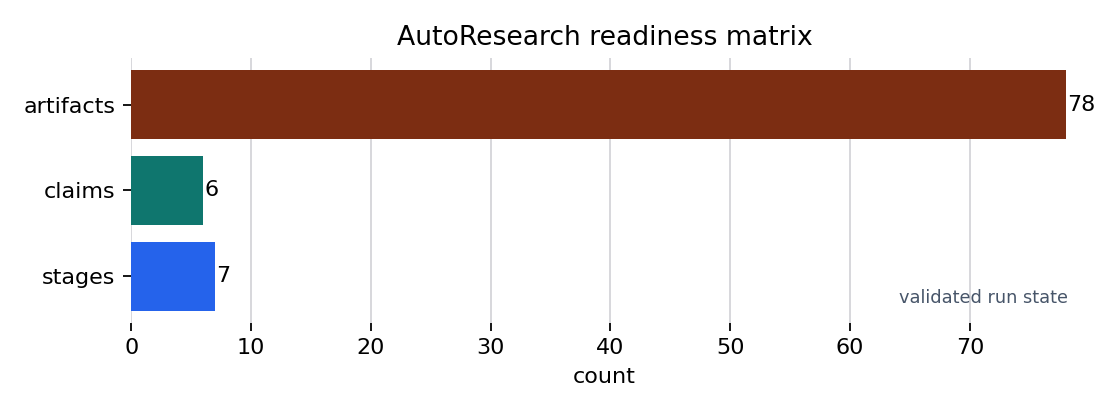
\includegraphics[keepaspectratio,alt={Validated AutoResearch run with 7 stages, 6 supported claims, and 78 required artifacts from output/data/autoresearch\_loop.json; the count summarizes readiness artifacts, not human approval. Generation method: Horizontal count summary from final loop metrics. Registry metadata records the generation method, source artifact, and claim boundary for validation.}]{../figures/autoresearch_stage_matrix.png}}
\caption{Validated AutoResearch run with 7 stages, 6 supported claims,
and 78 required artifacts from output/data/autoresearch\_loop.json; the
count summarizes readiness artifacts, not human approval. Generation
method: Horizontal count summary from final loop metrics. Registry
metadata records the generation method, source artifact, and claim
boundary for validation.}\label{fig:autoresearch_stage_matrix}
\end{figure}

\begin{figure}
\centering
\pandocbounded{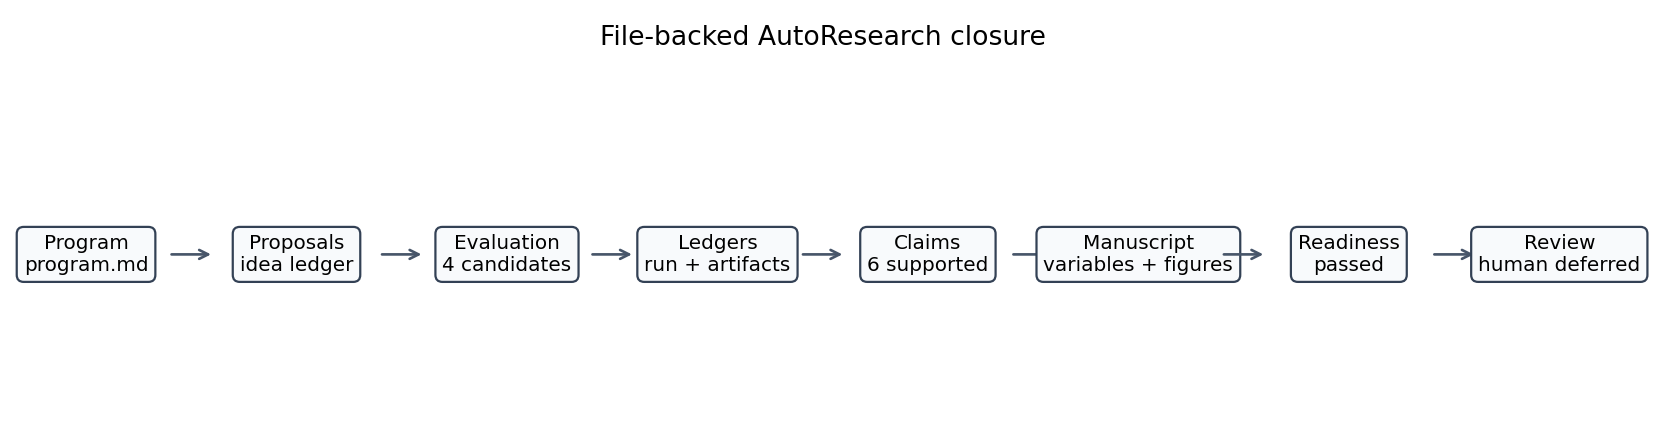
\includegraphics[keepaspectratio,alt={File-backed AutoResearch closure from program through review, with 6 supported claims and readiness passed; review remains a deferred human decision and the provenance path remains inspectable. Generation method: File-backed process-flow diagram from final loop state. Registry metadata records the generation method, source artifact, and claim boundary for validation.}]{../figures/autoresearch_closure_flow.png}}
\caption{File-backed AutoResearch closure from program through review,
with 6 supported claims and readiness passed; review remains a deferred
human decision and the provenance path remains inspectable. Generation
method: File-backed process-flow diagram from final loop state. Registry
metadata records the generation method, source artifact, and claim
boundary for validation.}\label{fig:autoresearch_closure_flow}
\end{figure}

\begin{longtable}[]{@{}
  >{\raggedright\arraybackslash}p{(\linewidth - 4\tabcolsep) * \real{0.3333}}
  >{\raggedright\arraybackslash}p{(\linewidth - 4\tabcolsep) * \real{0.3333}}
  >{\raggedright\arraybackslash}p{(\linewidth - 4\tabcolsep) * \real{0.3333}}@{}}
\caption{Generated artifact manifest from
\protect\breaktt{output/reports/artifact\_manifest.json}.}\label{tbl:autoresearch-loop}\tabularnewline
\toprule\noalign{}
\begin{minipage}[b]{\linewidth}\raggedright
Artifact
\end{minipage} & \begin{minipage}[b]{\linewidth}\raggedright
Role
\end{minipage} & \begin{minipage}[b]{\linewidth}\raggedright
Bytes
\end{minipage} \\
\midrule\noalign{}
\endfirsthead
\toprule\noalign{}
\begin{minipage}[b]{\linewidth}\raggedright
Artifact
\end{minipage} & \begin{minipage}[b]{\linewidth}\raggedright
Role
\end{minipage} & \begin{minipage}[b]{\linewidth}\raggedright
Bytes
\end{minipage} \\
\midrule\noalign{}
\endhead
output/data/autoresearch\_claims.json & Loop artifact & 1766 \\
output/data/autoresearch\_evidence\_overview.json & Evidence registry &
4436 \\
output/data/autoresearch\_integrity\_attestation.json & Security
evidence & 22755 \\
output/data/autoresearch\_inventory\_export.json & Security evidence &
20203 \\
output/data/autoresearch\_loop.json & Loop artifact & 16085 \\
output/data/autoresearch\_phase\_ledger.json & Run or candidate ledger &
3779 \\
output/data/autoresearch\_plan.json & Loop artifact & 17361 \\
output/data/autoresearch\_review\_packet.json & Review packet & 16204 \\
output/data/autoresearch\_schema\_manifest.json & Loop artifact &
7226 \\
output/data/autoresearch\_security\_profile.json & Security evidence &
1537 \\
output/data/autoresearch\_stage\_matrix.csv & Loop artifact & 749 \\
output/data/autoresearch\_supply\_chain\_inventory.json & Security
evidence & 21459 \\
output/data/autoresearch\_threat\_model.json & Security evidence &
6370 \\
output/data/benchmark\_boundary.json & Benchmark grading & 2363 \\
output/data/benchmark\_scores.json & Benchmark grading & 621 \\
output/data/figure\_quality\_report.json & Loop artifact & 16040 \\
output/data/figure\_style.json & Loop artifact & 1117 \\
output/data/idea\_ledger.json & Run or candidate ledger & 5233 \\
output/data/manuscript\_figure\_blocks.json & Manuscript hydration &
13062 \\
output/data/manuscript\_variable\_provenance.json & Manuscript hydration
& 30891 \\
output/data/manuscript\_variables.json & Manuscript hydration & 54968 \\
output/data/ml\_bootstrap\_intervals.json & Loop artifact & 615 \\
output/data/ml\_calibration\_bin\_intervals.json & Loop artifact &
2879 \\
output/data/ml\_calibration\_report.json & Loop artifact & 2201 \\
output/data/ml\_candidate\_intervals.json & Loop artifact & 1577 \\
output/data/ml\_candidate\_ledger.json & Run or candidate ledger &
570872 \\
output/data/ml\_candidate\_rank\_stability.json & Loop artifact &
3135 \\
output/data/ml\_candidate\_selection\_audit.json & Loop artifact &
2145 \\
output/data/ml\_class\_balance.json & Loop artifact & 2393 \\
output/data/ml\_classification\_diagnostics.json & Loop artifact &
4246 \\
output/data/ml\_confusion\_matrix.csv & Loop artifact & 271 \\
output/data/ml\_diagnostic\_boundary.json & Loop artifact & 2064 \\
output/data/ml\_error\_examples.json & Loop artifact & 989 \\
output/data/ml\_paired\_comparison.json & Loop artifact & 470 \\
output/data/ml\_prediction\_records.json & Loop artifact & 989913 \\
output/data/ml\_probability\_diagnostics.json & Loop artifact & 3045 \\
output/data/ml\_robustness\_report.json & Loop artifact & 3758 \\
output/data/ml\_statistical\_summary.json & Loop artifact & 3032 \\
output/data/ml\_task\_results.json & Loop artifact & 703566 \\
output/data/ml\_training\_diagnostics.json & Loop artifact & 2968 \\
output/data/ml\_training\_history.csv & Loop artifact & 6775 \\
output/data/mnist\_task\_config.json & Loop artifact & 3926 \\
output/data/research\_object\_manifest.json & Loop artifact & 20789 \\
output/data/research\_program.json & Loop artifact & 965 \\
output/data/review\_decisions.json & Review packet & 669 \\
output/data/run\_ledger.json & Run or candidate ledger & 328 \\
output/figures/autoresearch\_candidate\_lifecycle.png & Generated figure
& 28053 \\
output/figures/autoresearch\_closure\_flow.png & Generated figure &
40410 \\
output/figures/autoresearch\_integrity\_chain.png & Generated figure &
48256 \\
output/figures/autoresearch\_security\_control\_matrix.png & Generated
figure & 86574 \\
output/figures/ml\_bootstrap\_intervals.png & Generated figure &
21834 \\
output/figures/ml\_calibration\_reliability.png & Generated figure &
73889 \\
output/figures/ml\_candidate\_rank\_stability.png & Generated figure &
43692 \\
output/figures/ml\_candidate\_scores.png & Generated figure & 59953 \\
output/figures/ml\_classification\_metrics\_heatmap.png & Generated
figure & 55092 \\
output/figures/ml\_complexity\_accuracy.png & Generated figure &
35135 \\
output/figures/ml\_confusion\_matrix.png & Generated figure & 65820 \\
output/figures/ml\_confusion\_pairs.png & Generated figure & 33982 \\
output/figures/ml\_generalization\_gap.png & Generated figure & 48512 \\
output/figures/ml\_learning\_curves.png & Generated figure & 59258 \\
output/figures/ml\_paired\_correctness.png & Generated figure & 43309 \\
output/figures/ml\_per\_class\_accuracy.png & Generated figure &
34800 \\
output/figures/ml\_probability\_margin\_distribution.png & Generated
figure & 41754 \\
output/figures/ml\_probability\_quality.png & Generated figure &
38071 \\
output/figures/ml\_robustness\_matrix.png & Generated figure & 51332 \\
output/figures/ml\_selective\_accuracy.png & Generated figure & 48274 \\
output/figures/ml\_training\_dynamics.png & Generated figure & 51004 \\
output/figures/mnist\_class\_balance.png & Generated figure & 27059 \\
output/figures/mnist\_error\_examples.png & Generated figure & 28431 \\
output/figures/mnist\_subset\_contact\_sheet.png & Generated figure &
23617 \\
output/reports/autoresearch\_evidence\_overview.md & Evidence registry &
1136 \\
output/reports/autoresearch\_loop.json & Loop artifact & 16085 \\
output/reports/autoresearch\_review\_packet.md & Review packet & 912 \\
output/reports/autoresearch\_security\_review.md & Review packet &
1104 \\
output/reports/autoresearch\_summary.md & Loop artifact & 255 \\
output/reports/benchmark\_readiness\_smoke.json & Benchmark grading &
778 \\
output/reports/ml\_benchmark\_score.json & Benchmark grading & 382 \\
output/reports/ml\_experiment\_report.md & Loop artifact & 1687 \\
\bottomrule\noalign{}
\end{longtable}

\begin{longtable}[]{@{}
  >{\raggedright\arraybackslash}p{(\linewidth - 6\tabcolsep) * \real{0.2500}}
  >{\raggedright\arraybackslash}p{(\linewidth - 6\tabcolsep) * \real{0.2500}}
  >{\raggedright\arraybackslash}p{(\linewidth - 6\tabcolsep) * \real{0.2500}}
  >{\raggedright\arraybackslash}p{(\linewidth - 6\tabcolsep) * \real{0.2500}}@{}}
\caption{Review-gate decisions from
\protect\breaktt{output/data/review\_decisions.json}.}\label{tbl:review-gates}\tabularnewline
\toprule\noalign{}
\begin{minipage}[b]{\linewidth}\raggedright
Gate
\end{minipage} & \begin{minipage}[b]{\linewidth}\raggedright
Required
\end{minipage} & \begin{minipage}[b]{\linewidth}\raggedright
Decision
\end{minipage} & \begin{minipage}[b]{\linewidth}\raggedright
Rationale
\end{minipage} \\
\midrule\noalign{}
\endfirsthead
\toprule\noalign{}
\begin{minipage}[b]{\linewidth}\raggedright
Gate
\end{minipage} & \begin{minipage}[b]{\linewidth}\raggedright
Required
\end{minipage} & \begin{minipage}[b]{\linewidth}\raggedright
Decision
\end{minipage} & \begin{minipage}[b]{\linewidth}\raggedright
Rationale
\end{minipage} \\
\midrule\noalign{}
\endhead
proposal\_review & True & deferred & Decision is read from
human\_review.yaml when present; generated readiness is not approval. \\
evidence\_review & True & deferred & Decision is read from
human\_review.yaml when present; generated readiness is not approval. \\
\bottomrule\noalign{}
\end{longtable}

\begin{longtable}[]{@{}
  >{\raggedright\arraybackslash}p{(\linewidth - 6\tabcolsep) * \real{0.2500}}
  >{\raggedright\arraybackslash}p{(\linewidth - 6\tabcolsep) * \real{0.2500}}
  >{\raggedright\arraybackslash}p{(\linewidth - 6\tabcolsep) * \real{0.2500}}
  >{\raggedright\arraybackslash}p{(\linewidth - 6\tabcolsep) * \real{0.2500}}@{}}
\caption{Benchmark grading table from
\protect\breaktt{output/data/benchmark\_scores.json}.}\label{tbl:benchmark-scores}\tabularnewline
\toprule\noalign{}
\begin{minipage}[b]{\linewidth}\raggedright
Benchmark task
\end{minipage} & \begin{minipage}[b]{\linewidth}\raggedright
Status
\end{minipage} & \begin{minipage}[b]{\linewidth}\raggedright
Score
\end{minipage} & \begin{minipage}[b]{\linewidth}\raggedright
Grading output
\end{minipage} \\
\midrule\noalign{}
\endfirsthead
\toprule\noalign{}
\begin{minipage}[b]{\linewidth}\raggedright
Benchmark task
\end{minipage} & \begin{minipage}[b]{\linewidth}\raggedright
Status
\end{minipage} & \begin{minipage}[b]{\linewidth}\raggedright
Score
\end{minipage} & \begin{minipage}[b]{\linewidth}\raggedright
Grading output
\end{minipage} \\
\midrule\noalign{}
\endhead
readiness-smoke & graded & 1 &
output/reports/benchmark\_readiness\_smoke.json \\
ml-loop-score & graded & 1 & output/reports/ml\_benchmark\_score.json \\
\bottomrule\noalign{}
\end{longtable}

\begin{longtable}[]{@{}
  >{\raggedright\arraybackslash}p{(\linewidth - 8\tabcolsep) * \real{0.2000}}
  >{\raggedright\arraybackslash}p{(\linewidth - 8\tabcolsep) * \real{0.2000}}
  >{\raggedright\arraybackslash}p{(\linewidth - 8\tabcolsep) * \real{0.2000}}
  >{\raggedright\arraybackslash}p{(\linewidth - 8\tabcolsep) * \real{0.2000}}
  >{\raggedright\arraybackslash}p{(\linewidth - 8\tabcolsep) * \real{0.2000}}@{}}
\caption{Deterministic phase ledger from
\protect\breaktt{output/data/autoresearch\_phase\_ledger.json};
settlement order is not an autonomy
claim.}\label{tbl:phase-ledger}\tabularnewline
\toprule\noalign{}
\begin{minipage}[b]{\linewidth}\raggedright
Phase
\end{minipage} & \begin{minipage}[b]{\linewidth}\raggedright
Order
\end{minipage} & \begin{minipage}[b]{\linewidth}\raggedright
Group
\end{minipage} & \begin{minipage}[b]{\linewidth}\raggedright
Observed artifacts
\end{minipage} & \begin{minipage}[b]{\linewidth}\raggedright
Description
\end{minipage} \\
\midrule\noalign{}
\endfirsthead
\toprule\noalign{}
\begin{minipage}[b]{\linewidth}\raggedright
Phase
\end{minipage} & \begin{minipage}[b]{\linewidth}\raggedright
Order
\end{minipage} & \begin{minipage}[b]{\linewidth}\raggedright
Group
\end{minipage} & \begin{minipage}[b]{\linewidth}\raggedright
Observed artifacts
\end{minipage} & \begin{minipage}[b]{\linewidth}\raggedright
Description
\end{minipage} \\
\midrule\noalign{}
\endhead
intrinsic readiness & 1 & readiness & 3 & validate configured
project-intrinsic contracts \\
core artifacts & 2 & loop & 0 & write plan, stage matrix, and
provisional loop outputs \\
evidence registry & 3 & evidence & 2 & write local evidence registry \\
ml task & 4 & ml & 54 & run fixed-seed bounded candidate evaluation \\
method contract & 5 & governance & 3 & write program, idea, run, review,
and benchmark ledgers \\
provisional payloads & 6 & settlement & 12 & refresh loop payloads
before extrinsic validation \\
security artifacts & 7 & security & 10 & write local security and
integrity evidence \\
final visuals & 8 & figures & 54 & write final registry-backed
figures \\
manuscript hydration & 9 & manuscript & 9 & write variables, provenance,
and figure blocks \\
readiness manifest & 10 & settlement & 12 & refresh checksum manifest
before extrinsic validation \\
schema manifest & 11 & schema & 2 & write generated JSON schema-version
manifest \\
research object manifest & 12 & packaging & 2 & write local
research-object manifest \\
extrinsic readiness & 13 & readiness & 3 & validate generated artifacts
and extrinsic contracts \\
final schema manifest & 14 & schema & 2 & refresh schema manifest after
final payload updates \\
final research object manifest & 15 & packaging & 2 & refresh local
research-object manifest \\
artifact manifest & 16 & settlement & 12 & write final artifact checksum
manifest \\
\bottomrule\noalign{}
\end{longtable}

\begin{longtable}[]{@{}
  >{\raggedright\arraybackslash}p{(\linewidth - 8\tabcolsep) * \real{0.2000}}
  >{\raggedright\arraybackslash}p{(\linewidth - 8\tabcolsep) * \real{0.2000}}
  >{\raggedright\arraybackslash}p{(\linewidth - 8\tabcolsep) * \real{0.2000}}
  >{\raggedright\arraybackslash}p{(\linewidth - 8\tabcolsep) * \real{0.2000}}
  >{\raggedright\arraybackslash}p{(\linewidth - 8\tabcolsep) * \real{0.2000}}@{}}
\caption{Figure-quality checks from
\protect\breaktt{output/data/figure\_quality\_report.json}; 25 registered
figure(s) were checked.}\label{tbl:figure-quality}\tabularnewline
\toprule\noalign{}
\begin{minipage}[b]{\linewidth}\raggedright
Figure
\end{minipage} & \begin{minipage}[b]{\linewidth}\raggedright
Pixels
\end{minipage} & \begin{minipage}[b]{\linewidth}\raggedright
Variance
\end{minipage} & \begin{minipage}[b]{\linewidth}\raggedright
Source exists
\end{minipage} & \begin{minipage}[b]{\linewidth}\raggedright
Nonblank
\end{minipage} \\
\midrule\noalign{}
\endfirsthead
\toprule\noalign{}
\begin{minipage}[b]{\linewidth}\raggedright
Figure
\end{minipage} & \begin{minipage}[b]{\linewidth}\raggedright
Pixels
\end{minipage} & \begin{minipage}[b]{\linewidth}\raggedright
Variance
\end{minipage} & \begin{minipage}[b]{\linewidth}\raggedright
Source exists
\end{minipage} & \begin{minipage}[b]{\linewidth}\raggedright
Nonblank
\end{minipage} \\
\midrule\noalign{}
\endhead
fig:autoresearch\_candidate\_lifecycle & 1184x480 & 0.083 & True &
True \\
fig:autoresearch\_closure\_flow & 1664x448 & 0.015 & True & True \\
fig:autoresearch\_integrity\_chain & 1440x734 & 0.040 & True & True \\
fig:autoresearch\_security\_control\_matrix & 1470x734 & 0.014 & True &
True \\
fig:autoresearch\_stage\_matrix & 1120x416 & 0.080 & True & True \\
fig:ml\_bootstrap\_intervals & 1152x448 & 0.009 & True & True \\
fig:ml\_calibration\_reliability & 1152x832 & 0.015 & True & True \\
fig:ml\_candidate\_rank\_stability & 1408x608 & 0.053 & True & True \\
fig:ml\_candidate\_scores & 1376x688 & 0.013 & True & True \\
fig:ml\_classification\_metrics\_heatmap & 928x832 & 0.092 & True &
True \\
fig:ml\_complexity\_accuracy & 1120x608 & 0.010 & True & True \\
fig:ml\_confusion\_matrix & 896x768 & 0.046 & True & True \\
fig:ml\_confusion\_pairs & 1152x576 & 0.129 & True & True \\
fig:ml\_generalization\_gap & 1184x864 & 0.059 & True & True \\
fig:ml\_learning\_curves & 1216x608 & 0.018 & True & True \\
fig:ml\_paired\_correctness & 768x672 & 0.075 & True & True \\
fig:ml\_per\_class\_accuracy & 1152x512 & 0.098 & True & True \\
fig:ml\_probability\_margin\_distribution & 1184x864 & 0.024 & True &
True \\
fig:ml\_probability\_quality & 1344x608 & 0.046 & True & True \\
fig:ml\_robustness\_matrix & 1280x608 & 0.073 & True & True \\
fig:ml\_selective\_accuracy & 1088x608 & 0.016 & True & True \\
fig:ml\_training\_dynamics & 1408x608 & 0.072 & True & True \\
fig:mnist\_class\_balance & 1216x544 & 0.071 & True & True \\
fig:mnist\_error\_examples & 1280x734 & 0.234 & True & True \\
fig:mnist\_subset\_contact\_sheet & 1216x544 & 0.228 & True & True \\
\bottomrule\noalign{}
\end{longtable}
\end{frame}

\begin{frame}[fragile,allowframebreaks]{Security Readiness And Integrity
Evidence}
\protect\phantomsection\label{sec:security-readiness-integrity}
The local security profile reports attestation status \texttt{passed}
after checking \texttt{80} file record(s), with \texttt{0} missing
record(s) and \texttt{0} checksum mismatch(es). The inventory contains
\texttt{14} input record(s) and \texttt{69} generated-artifact
record(s). The integrity-chain figure is
@fig:autoresearch\_integrity\_chain. These values support local
artifact-integrity claims only; they do not claim external signing,
production SLSA compliance, or runtime security monitoring.

\begin{figure}
\centering
\pandocbounded{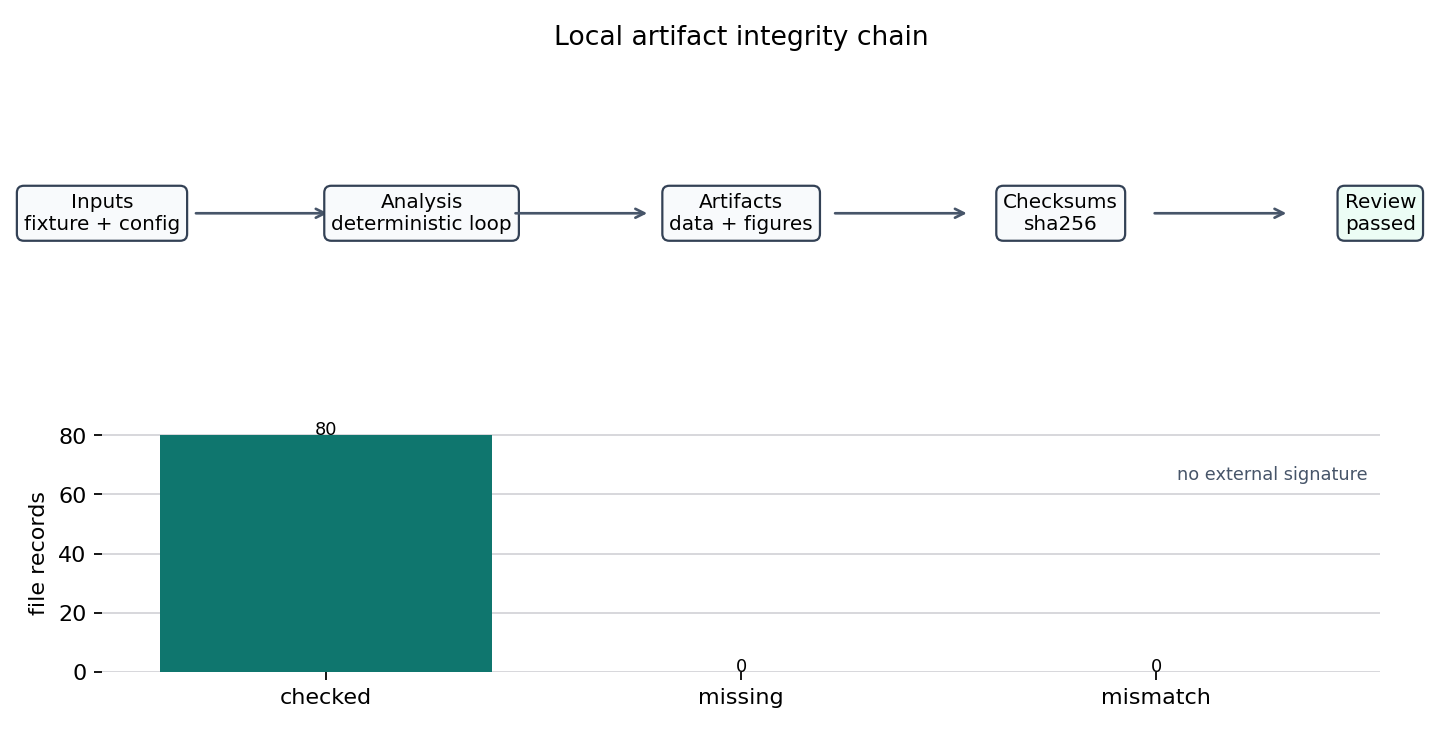
\includegraphics[keepaspectratio,alt={Local integrity chain from output/data/autoresearch\_integrity\_attestation.json; checksums summarize the observed run artifacts and remain unsigned local evidence. Generation method: Local checksum attestation chain with checked, missing, and mismatch counts. Registry metadata records the generation method, source artifact, and claim boundary for validation.}]{../figures/autoresearch_integrity_chain.png}}
\caption{Local integrity chain from
output/data/autoresearch\_integrity\_attestation.json; checksums
summarize the observed run artifacts and remain unsigned local evidence.
Generation method: Local checksum attestation chain with checked,
missing, and mismatch counts. Registry metadata records the generation
method, source artifact, and claim boundary for
validation.}\label{fig:autoresearch_integrity_chain}
\end{figure}

\begin{longtable}[]{@{}ll@{}}
\caption{Integrity-attestation summary from
\protect\breaktt{output/data/autoresearch\_integrity\_attestation.json}.}\label{tbl:security-integrity}\tabularnewline
\toprule\noalign{}
Integrity field & Value \\
\midrule\noalign{}
\endfirsthead
\toprule\noalign{}
Integrity field & Value \\
\midrule\noalign{}
\endhead
status & passed \\
algorithm & sha256 \\
checked files & 80 \\
missing files & 0 \\
checksum mismatches & 0 \\
external signature & False \\
\bottomrule\noalign{}
\end{longtable}
\end{frame}

\begin{frame}[fragile,allowframebreaks]{Manuscript Hydration Provenance}
\protect\phantomsection\label{sec:manuscript-hydration-provenance}
The final run supports \texttt{6} manuscript-facing claim(s) and checks
\texttt{78} required artifact(s). The rendered manuscript uses injected
variables from generated data payloads, so the abstract and results
track the latest analysis run rather than hard-coded counts. The final
readiness status is \texttt{passed}; generated review decisions are
recorded as deferred for human review rather than as self-approval.

\begin{longtable}[]{@{}ll@{}}
\caption{Variable provenance summary from
\protect\breaktt{output/data/manuscript\_variable\_provenance.json}.}\label{tbl:variable-provenance}\tabularnewline
\toprule\noalign{}
Source artifact & Injected variables or fragments \\
\midrule\noalign{}
\endfirsthead
\toprule\noalign{}
Source artifact & Injected variables or fragments \\
\midrule\noalign{}
\endhead
output/data/autoresearch\_integrity\_attestation.json & 5 \\
output/data/autoresearch\_loop.json & 57 \\
output/data/autoresearch\_phase\_ledger.json & 2 \\
output/data/autoresearch\_schema\_manifest.json & 1 \\
output/data/autoresearch\_security\_profile.json & 6 \\
output/data/autoresearch\_supply\_chain\_inventory.json & 3 \\
output/data/autoresearch\_threat\_model.json & 4 \\
output/data/benchmark\_scores.json & 1 \\
output/data/figure\_quality\_report.json & 3 \\
output/data/manuscript\_variable\_provenance.json & 1 \\
output/data/ml\_bootstrap\_intervals.json & 3 \\
output/data/ml\_calibration\_bin\_intervals.json & 1 \\
output/data/ml\_calibration\_report.json & 3 \\
output/data/ml\_candidate\_intervals.json & 1 \\
output/data/ml\_candidate\_ledger.json & 1 \\
output/data/ml\_candidate\_rank\_stability.json & 3 \\
output/data/ml\_candidate\_selection\_audit.json & 1 \\
output/data/ml\_class\_balance.json & 3 \\
output/data/ml\_classification\_diagnostics.json & 5 \\
output/data/ml\_diagnostic\_boundary.json & 1 \\
output/data/ml\_paired\_comparison.json & 3 \\
output/data/ml\_probability\_diagnostics.json & 4 \\
output/data/ml\_robustness\_report.json & 2 \\
output/data/ml\_statistical\_summary.json & 9 \\
output/data/ml\_task\_results.json & 39 \\
output/data/ml\_training\_diagnostics.json & 7 \\
output/data/research\_object\_manifest.json & 2 \\
output/data/review\_decisions.json & 1 \\
output/figures/figure\_registry.json & 51 \\
output/reports/artifact\_manifest.json & 1 \\
\bottomrule\noalign{}
\end{longtable}
\end{frame}

\end{document}
